% !TeX program = xelatex
% =====================================================================
%  论文正文草稿 —— 汇编壳
%  编译：xelatex draft_main.tex   （建议跑两遍以解析交叉引用）
%
%  正文按章拆分在 paper/sections/ 下，每个文件独立成章：
%    ch1_problem.tex     问题重述与分析
%    ch2_assumptions.tex 模型假设与符号说明
%    preprocess.tex      数据核验与预处理（沿用既有内容并补充数据核验表与零点还原表）
%    ch4_q1.tex          问题一：50 维感官评分预测
%    ch5_q2.tex          问题二：基于共表达图的关键化合物识别
%    ch6_q3.tex          问题三：风格条件生成、感官画像与跨风格迁移
%    ch7_evaluation.tex  模型评价与改进
%    ch8_conclusion.tex  结论与建议
%    references.tex      参考文献
%    appendix.tex        附录 A--F
%  每章可单独包装成独立文档编译（参考 paper/preprocess.tex 的壳）。
% =====================================================================
\documentclass[12pt,a4paper]{article}

\usepackage{ctex}
\usepackage{geometry}
\geometry{left=2.5cm,right=2.5cm,top=2.5cm,bottom=2.5cm}
\usepackage{amsmath,amssymb}
\usepackage{graphicx}
\usepackage{xcolor}
\usepackage{booktabs}
\usepackage{multirow}
\usepackage{array}
\usepackage{caption}
\usepackage{subcaption}
\usepackage{float}
\usepackage[colorlinks=true,linkcolor=black,citecolor=black]{hyperref}

\graphicspath{{../figures/}}
\setlength{\parskip}{0.45em}
\renewcommand{\arraystretch}{1.25}

\newcommand{\code}[1]{\texttt{#1}}

% 首页版式依据赛题论文模板：队伍编号/赛道表、分隔线、论文题目、摘要与关键词
\newcommand{\teaminfo}[2]{%
  \par\begingroup\centering
  \renewcommand{\arraystretch}{1.15}
  \begin{tabular}{|c|c|}
    \hline
    \makebox[3.9cm][c]{队伍编号} & \makebox[3.9cm][c]{#1} \\
    \hline
    \makebox[3.9cm][c]{赛道} & \makebox[3.9cm][c]{#2} \\
    \hline
  \end{tabular}
  \par\endgroup
}

% 摘要与正文同宽（默认 abstract 环境由 quotation 包裹，左右各缩进约 2.5em）
\makeatletter
\renewenvironment{abstract}{%
  \small
  \begin{center}{\bfseries 摘\quad 要}\end{center}%
  \par\vspace{0.5em}%
  \noindent\ignorespaces
}{\par}
\makeatother

\newcommand{\papertitle}{啤酒化学数据与感官评分}

\begin{document}

\vspace*{-0.5cm}
\teaminfo{MCB2607307}{（A）}

\vspace{0.15cm}
\noindent\textcolor{gray}{\rule{14.5cm}{1pt}}
\vspace{0.15cm}

{\centering\bfseries\large\papertitle\par}

\begin{abstract}
啤酒的风味品质由化学成分与感官品评共同刻画，但两者之间难以建立直接的定量关系。
本文基于一份含 250 款商用啤酒的化学与感官数据集，完成三项任务：由化学特征预测 50 个感官维度的 0 到 6 等级，找出每个感官维度的关键化合物，以及生成指定风格的化合物谱并完成跨风格迁移。

针对问题一，本文以作者公布的啤酒感官维度原始评分均分为训练目标，用浅层梯度提升树逐维拟合化学特征到该均分的映射。
按 25 个日期组分组的嵌套交叉验证评估对新啤酒的泛化能力，同日品评、共享品评员与品评情境的啤酒整体进入同一折以避免泄漏。
再由内层折外残差构造等级预测分布，分别以分布中位数、分位数切点等级为主要、第二输出。
主模型等级平均绝对误差为 0.479，显著低于只用风格预测的基线 0.527（配对差 $-0.048$，95\% 置信区间 $[-0.062,-0.034]$），二次加权 Kappa 为 0.290，90\% 等级区间覆盖 97.2\%。
使用附件四还原等级评分的对照端到端平均绝对误差为 0.786，说明标准化换算本身是主要误差来源。

针对问题二，本文以附件二构建化合物共表达图，在阈值 0.6 下用平均连接层次聚类划分模块，再用图约束前向选择逐个取出控制已选化合物后的秩偏相关最强、且分属不同模块的 3 个化合物。
显著性由置换检验把关，稳定性由 25 个日期组重抽 1,000 次量化。
维度按首位化合物的显著性与入选频率分档，A 级为首位显著且入选频率不低于 0.6，B 级为首位显著但不满足该条件，C 级为首位不显著；49 个维度中 A 级 26 个、B 级 22 个、C 级 1 个。

针对问题三，本文对化学数据做秩变换，用风格条件潜在高斯模型刻画化合物谱，以因子载荷与共表达模块块描述风格内共变，再经问题一模型给出感官画像。
跨风格迁移采用潜空间平移，配合化学层缺陷约束的投影与感官层的路径搜索，保证缺陷化合物不恶化。
原尺度复查指把迁移结果映回附件一原尺度、逐列核对缺陷化合物不超过上界且预测等级不升高，不通过者退回下一个可行网格点。
区分真实与生成化合物谱的两样本分类检验的合并与条件曲线下面积（AUC）为 0.589 与 0.576，超出 $|\mathrm{AUC}-0.5|\le 0.05$ 的预设标准，即生成谱与真实谱仍可被区分，但均低于去掉风格条件的对照；新颖性、分类可用性、下限比例误差与模块内相关等其余检验通过。

总体而言，化学谱对感官等级具有超出风格基线的预测能力，关键化合物识别具备可量化的稳定性，生成与迁移在缺陷约束下提供了可用的分析框架。
\end{abstract}

\noindent\textbf{关键词：}啤酒风味；感官评分预测；梯度提升树；化合物共表达网络；秩变换；条件生成模型；跨风格迁移

\clearpage
\tableofcontents
\newpage

\section{问题重述与分析}

\subsection{研究背景与任务要求}

赛题提供一份商用啤酒风味数据集，包含八份附件。
附件一记录 250 款啤酒的 231 个化学与理化特征，附件二给出这些特征两两之间的相关系数矩阵。
附件三定义感官记分卡，附件四给出 250 款啤酒在 50 个感官维度上的标准化品评小组均值。
附件八补充部分化合物的校准浓度、气味阈值、来源标签与缺陷描述。
这些附件对应 Schreurs 等人在 \emph{Nature Communications} 发表的数据记录，作者在同一数据记录的新版中另行公布了逐品评员、逐啤酒的原始 0 到 6 分评分，覆盖相同的 250 款啤酒，是三个问题的感官数据来源。

赛题要求完成三项任务。
问题一以化学数据预测啤酒的感官评分，问题二找出每个感官维度的关键化合物，问题三生成指定风格的一款啤酒在各化学特征上的取值向量，即化合物谱，并进行跨风格迁移。

\subsection{问题分析}

\subsubsection{评分预测}

问题一从化学特征预测每款啤酒在每个感官维度上的品评等级。
对啤酒 $b$（$b=1,\dots,250$）与感官维度 $d$（$d=1,\dots,50$），把该啤酒该维度的全部原始评分记录取算术平均得到 $\bar x_{bd}$，再截断到 0 到 6 并四舍五入，得到等级 $G_{bd}$。
交付物为每款啤酒每个维度的预测等级、等级概率与 90\% 等级区间。
难点在于样本量小、特征维数高：附件一的化学数据有缺失值，待评分的新啤酒没有任何品评记录，评分只能由化学数据预测；感官评分还含品评员之间的系统差异与随机噪声，同一天品评的啤酒共享出席名单与品评情境，不能当作相互独立的样本。
因此既要在训练折内处理化学缺失，又要用按日期组分组的嵌套交叉验证控制同日信息泄漏。

\subsubsection{化合物识别}

问题二的目标是找出每个感官维度上关联最强的三个化合物。
第 1 位取与维度秩相关最强的化合物，第 2、3 位在控制已选化合物之后取秩偏相关最强、且不属于已选化合物所在共表达模块的化合物。
这一目标把关键化合物定义为关联结果，而不是因果结果，附件中没有干预数据，化学合理性在结果产生后另行解释。
难点在于附件二只在全部 250 款啤酒上估计两两相关，风格之间的配方差异与风格内的共变混在一起；同一模块内的化合物高度相关，边际关联最强的几个化合物往往来自同一模块，直接取前 3 会重复选择同一条信息。
因此需要先用模拟还原实验确定选择规则，再用日期组重抽量化入选频率。

\subsubsection{风格生成}

问题三的估计目标有三项：风格条件分布、感官画像与迁移映射。
风格条件分布是给定细分风格后 225 个生成列的联合分布，感官画像是由该分布生成的化合物谱经问题一模型得到的 50 维等级分布，迁移映射是把一种风格的化合物谱改为另一种风格、同时满足化学层与感官层两层缺陷约束。
难点在于 22 个细分风格中每个只有 3 到 31 款啤酒，少于 225 个生成列，风格专属的完整协方差不可估计；生成结果既要落在观测范围内，又要让风格判别器无法区分生成样本与真实啤酒，还不能只是复制训练啤酒；迁移时题面要求缺陷化合物不恶化，需要写成可检验的约束，并在潜空间与原始尺度两处复查。

三项任务共享同一批啤酒与化学特征，按问题一、问题二、问题三的顺序衔接，前两问的产物作为第三问的输入。
问题一建立化学谱到 50 维感官评分分布的映射；问题二借助共表达模块识别每个感官维度的关键化合物候选；问题三建立以风格为条件的生成模型，调用问题一的评分映射形成感官画像，并在化学与感官两层约束下完成跨风格迁移。

\section{模型假设与符号说明}

\subsection{模型假设}

假设 1：化学测量是每款啤酒的稳定属性，不随品评日期或品评场次变化。
化学量由仪器测定，与品评场次无关，每款啤酒因此对应唯一的化学谱。
据此化学谱可以按风格分层划分验证折，感官标签则须按日期组划分。
问题一以 250 款化学谱预测感官评分，问题二在化学与感官之间建立关联，问题三的生成模型按风格分层。

<<<<<<< HEAD
\begin{table}[htbp]
\centering\small
\caption{全局假设}
\label{tab:assumptions}
\begin{tabular}{>{\raggedright\arraybackslash}p{3.4cm}>{\raggedright\arraybackslash}p{4.6cm}>{\raggedright\arraybackslash}p{4.6cm}}
\toprule
假设 & 理由 & 对模型的影响 \\
\midrule
样本对齐以行号为准 & 原始评分文件中的编号对应附件一、四的行号，按行号对齐时逐维 Spearman 中位数为 0.969，按附件列对齐为 $-0.010$ & 所有连接都按行号，交叉验证分组与感官目标随之对齐 \\
\addlinespace
未校准信号列按 $\log_{10}$ 相对峰面积解释 & 157 个色谱质谱列没有绝对浓度校准数据，无法逐列证实底数 & 梯度提升树模型直接使用发布值，其分裂顺序不受底数选择影响；需要浓度时用 $10^x$ 还原 \\
\addlinespace
共同下限按未检出状态处理 & 142 列共 6,807 个单元等于共同下限 $-1.81781854$，现有材料不能确认仪器检出限 & 树模型把该值作为最低秩，线性模型加逐列下限指示变量 \\
\addlinespace
化学缺失值以训练折列均值填充 & 缺失只有 73 个单元，删去含缺失啤酒会损失 25.2\% 的样本 & 填充值只作计算占位，不解释为真实零或未检出 \\
\addlinespace
感官目标为当次出席品评员的平均分 & 加性模型中出席名单带来的偏移占啤酒间方差的中位数只有 2.2\% & 目标不校正出席名单差异，敏感性分析另行检验 \\
\addlinespace
细分风格标签准确 & 赛题以该标签作为问题三的条件变量 & 生成器按标签学习风格条件分布，不合并相近风格 \\
\addlinespace
文献气味阈值在啤酒基质中成立 & 阈值取自附件八的感官阈值 & 只有气味活度值的计算与迁移阈值依赖该假设 \\
\bottomrule
\end{tabular}
\end{table}
=======
假设 2：感官评分在同一品评日期组内相关，日期组是相关与独立性的单位。
同一日期组的啤酒共享品评员与品评情境，有各自的噪声、偏差与评分习惯。
因此交叉验证、重抽样与留出验证都以日期组为单位，问题一使用按日期组分组的嵌套交叉验证，问题二使用日期组簇 bootstrap，问题三的画像验证按日期组划分。
>>>>>>> 28f0f3593e345d7e82eeec8b19294d46c1357145

假设 3：分析范围限于观测到的化学取值，不向外推。
观测范围之外的取值没有数据支持，基于树的模型在范围外只能做常数外推。
因此生成与迁移输出的化合物谱被限制在观测范围内，超出范围的取值不作为结论依据。

假设 4：附件八的缺陷阈值单位与附件一对应列一致。
对数列的阈值取常用对数值，线性列的阈值取原值，阈值与化学列必须同尺度才可比。
这一假设决定化学层缺陷上界与超阈比例，迁移中另以不依赖阈值与单位的严格不增加规则作为对照。

\subsection{符号定义}

跨问题共用的符号列于表~\ref{tab:symbols}。
方法局部的符号在引入它们的一节定义，不在此列出。

\begin{table}[htbp]
\centering\small
\caption{共用符号}
\label{tab:symbols}
\begin{tabular}{cll}
\toprule
符号 & 含义 & 单位 \\
\midrule
$b$ & 啤酒索引，$b=1,\dots,250$ & 无 \\
$d$ & 感官维度，附件四的 50 列之一，$d=1,\dots,50$ & 无 \\
$X_b$ & 啤酒 $b$ 的化学特征，即附件一的 231 列 & 混合，见数据审计 \\
$\bar x_{bd}$ & 啤酒 $b$ 在维度 $d$ 上的品评小组原始评分均值 & 0--6 分 \\
$z_{bd}$ & 附件四标准化后的品评小组评分 & 以每位品评员标准差为单位 \\
$s(b)$ & 啤酒 $b$ 的细分风格标签，共 22 类 & 无 \\
\bottomrule
\end{tabular}
\end{table}

$\bar x_{bd}$ 是问题一与问题二的感官目标，也是问题三感官画像的观测真值。
$z_{bd}$ 是 $\bar x_{bd}$ 的确定性标准化，按品评员与维度标准化后再对小组取平均，去掉 0 到 6 量表的均值与标准差，只在数据核对、仅用附件的对照与问题二的敏感性分析中使用。
$s(b)$ 是问题三的条件变量，也是问题一基线所要超越的信息来源。

\section{数据预处理}

建模之前，首先对 8 个附件的规模、标识列与取值口径做统一核查，并完成缺失值填充、异常值判定、对数底数核验与评分量纲还原四项工作。本章的全部数值均由原始附件直接统计得到，未引入任何外部数据。

\subsection{数据概览与一致性核查}

本赛题提供的附件涵盖化合物丰度、化合物间相关性、感官记分卡、标准化感官面板与理化参数等多个层面，其规模与缺失情况如表~\ref{tab:overview} 所示。

\begin{table}[H]\centering\small
\caption{各附件数据概览与缺失情况}\label{tab:overview}
\begin{tabular}{llccrr}
\toprule
附件 & 内容 & 规模（样本$\times$列） & 有效测量变量 & 缺失单元格 & 缺失率 \\
\midrule
1 (\code{1.csv})  & 化合物丰度矩阵   & $250\times234$ & 231 &   73 & 0.125\% \\
2 (\code{2.csv})  & 化合物相关矩阵   & $231\times232$ & 231 &    0 & 0       \\
3 (\code{3.xlsx}) & 感官记分卡       & 12 张记分卡    & 50  & ---  & ---     \\
4 (\code{4.csv})  & 标准化感官评分   & $250\times53$  &  50 &    0 & 0       \\
7 (\code{7.csv})  & 感官属性面板     & $250\times189$ & 183 &  750 & 1.59\%  \\
\bottomrule
\end{tabular}
\end{table}

核查中有三点需专门说明。

\textbf{第一，样本量口径。}题面正文提及``226 种啤酒''，但实测附件1、附件4、附件7 的样本行数均为 250。两者不一致，且无法由数据本身调和，故本研究一律以实测的 $n=250$ 为准，并在全文保持该口径；题面数字仅在讨论中提及，不参与任何计算。

\textbf{第二，变量列数口径。}附件1 共 234 列，剔除 \code{beer}、\code{beer\_id} 与 \code{tasting\_category\_fine} 三个标识/分类列后，有效测量变量为 231 个；附件2 的相关性矩阵恰为 $231\times231$，与之\textbf{完全对应}。这说明两份附件的变量口径一致，可直接联用而无需对齐映射——附件2 的行序与附件1 的测量列序一一对应，是后续构建共表达网络的前提。

\textbf{第三，附件7 的列构成。}189 列中，3 列为标识与风格标签，另有 3 列为全空列（详见缺失值填充一小节），故有效测量变量为 183 个，全部为数值型感官属性。此外，附件3 汇总表所列的 50 个感官变量与附件4 的 50 个数值列\textbf{一一对应}：前者给出 0--6 原始记分及其记分规则，后者为 250 个样本的标准化面板，二者共同构成问题一的目标变量。

\subsection{缺失值填充}

\subsubsection{缺失情况的定位}

对主要数值附件逐单元格扫描，得到附件1 的 73 个空值集中于 9 个化合物变量，明细见表~\ref{tab:miss1} 与图~\ref{fig:miss}。

\begin{table}[H]\centering\small
\caption{附件1 中存在缺失的化合物变量}\label{tab:miss1}
\begin{tabular}{lrr}
\toprule
变量 & 缺失个数 & 占 250 个样本的比例 \\
\midrule
\code{amyl.acetate}          & 27 & 10.8\% \\
\code{aroma\_hops\_sum}      & 13 &  5.2\% \\
\code{methylpyrazine}        & 12 &  4.8\% \\
\code{X2.3.butanedione}      &  9 &  3.6\% \\
\code{X3.methylbutanal}      &  7 &  2.8\% \\
\code{ethyl.nicotinate}      &  2 &  0.8\% \\
\code{ethyl.isobutyrate}     &  1 &  0.4\% \\
\code{furfural}              &  1 &  0.4\% \\
\code{phenylacetaldehyde}    &  1 &  0.4\% \\
\midrule
合计 & 73 & --- \\
\bottomrule
\end{tabular}
\end{table}

\begin{figure}[H]\centering
\includegraphics[width=0.98\textwidth]{fig_missing.png}
\caption{附件1 缺失值分布}\label{fig:miss}
\end{figure}

图~\ref{fig:miss}(b) 显示，缺失位置沿样本轴近似均匀散布，未出现按样本成片缺失或按变量成段缺失的情形。这说明缺失并非由某一批次测量整体失败引起，而更接近逐次进样的偶发失效。该观察支持``逐变量建模填补''而非``整行删除''的策略：若删除含缺失的样本，仅 \code{amyl.acetate} 一项即损失 27 个样本点，且缺失集中在特定样本区间，会造成风格分布偏移。

\subsubsection{附件7 的全空列处理}

附件7 的 \code{palate\_acetaldehyde}、\code{palate\_acetate}、\code{palate\_dentist} 三个列在全部 250 个样本上均为空（各 250 个 NA，合计 750 个）。对缺失率达 100\% 的变量，任何插补算法都只能凭空生成数据，其输出完全由模型先验决定而不含任何观测信息。因此本研究\textbf{直接剔除}这三个列，不纳入后续建模，并在结果讨论中注明。

\subsubsection{填补模型：浅层梯度提升树}

题面要求``从化学成分出发还原 0--6 评分''，因此缺失填补不应是孤立的统计插值，而应与下游的``化学成分 $\to$ 评分''映射共用同一套函数形式。为此，本研究以浅层梯度提升树作为填补模型。

设第 $j$ 个存在缺失的变量，其完整观测样本集为 $\mathcal{O}_j$，缺失样本集为 $\mathcal{M}_j$。以化学成分为输入 $\mathbf{x}_i\in\mathbb{R}^{p}$、标准化评分为目标，第 $m$ 轮的浅层回归树为 $f_m$，学习率为 $\eta$，则缺失位置的预测值为
\begin{equation}\label{eq:gbdt}
  \hat{y}^{(j)}_{i} \;=\; \sum_{m=1}^{M}\eta\, f_m(\mathbf{x}_i),
  \qquad i\in\mathcal{M}_j .
\end{equation}

式~\eqref{eq:gbdt} 的意义在于：该提升树一旦训练完成，即成为一个以化学成分为输入、标准化评分为输出的显式函数，既可用于补齐附件1 的 73 个空值，也可用于预测题面所要求的缺失评分，两者共用同一套参数，避免了``插补模型''与``预测模型''口径不一致的问题。

选择``浅层''（树深 $d\le 3$）而非深树，基于三点考虑：

\begin{enumerate}
\item 本数据 $n=250$ 而 $p\approx233$，样本量远小于特征数，深树极易记忆训练样本。限制树深相当于对模型复杂度施加显式正则。
\item 附件2 表明化合物之间存在显著共线性。线性插补（如回归插补、MICE 的线性条件模型）在共线设计下方差会被放大；树模型按特征逐一贪心切分，对共线性不敏感。
\item 化合物与感官评分之间多为\textbf{阈值型}关系——浓度越过感知阈值后评分才上升。树的阶梯函数形式比线性形式更贴合这一物理机制。
\end{enumerate}

为防止信息泄漏，式~\eqref{eq:gbdt} 的提升树在\textbf{每一个交叉验证折内重新拟合}：先在训练折上训练，再对验证折的缺失位置做预测；在全量数据上拟合的填补器不得用于任何评估环节。

\subsection{异常值的检测与处理}

\subsubsection{量纲归一与朴素判据}

附件4 与附件7 的变量取值区间差异极大，直接比较绝对偏差没有意义。参照通行做法，先做 Min--Max 归一化：
\begin{equation}\label{eq:minmax}
  X' \;=\; \frac{X - X_{\min}}{X_{\max} - X_{\min}} ,
\end{equation}
其中 $X$ 为原始数据，$X'$ 为归一化数据，$X_{\min}$、$X_{\max}$ 分别为该变量的最小值与最大值。随后用 Tukey 的 $1.5$ 倍四分位距规则初筛，即
\begin{equation}\label{eq:tukey}
  x_i \ \text{判为异常} \iff
  x_i \notin \big[\,Q_1 - 1.5\,\mathrm{IQR},\;\; Q_3 + 1.5\,\mathrm{IQR}\,\big],
  \qquad \mathrm{IQR} = Q_3 - Q_1 .
\end{equation}
初筛结果见表~\ref{tab:outlier}。

\begin{table}[H]\centering\small
\caption{朴素 Tukey 规则的初筛结果（已剔除标识列）}\label{tab:outlier}
\begin{tabular}{lrrrrr}
\toprule
数据表 & 数值列数 & 被标记样本数 & 标记率 & $\mathrm{IQR}=0$ 的列数 & 退化列占比 \\
\midrule
附件4 &  50 &  693 & 5.54\% &  0 &  0      \\
附件7 & 183 & 3899 & 8.52\% & 59 & 32.24\% \\
\bottomrule
\end{tabular}
\end{table}

\subsubsection{朴素判据的失效及其原因}

初筛结果暴露出一个必须处理的问题：附件7 的 183 个数值型感官维度中，有 59 个（32.24\%）满足 $Q_1 = Q_3$，即 $\mathrm{IQR} = 0$。

此时式~\eqref{eq:tukey} 的区间退化为单点 $[Q_3,\,Q_3]$，任何不等于该点的取值都会被判为异常。而这 59 个维度的分布形态属于典型的\textbf{零膨胀}：183 个维度中有 177 个（96.7\%）超过半数样本取地板值（对应 0--6 量表中的``不存在''）。于是 $Q_1 = Q_3 = f_j$（地板值），而所有真正被评委打过分的样本全部落在区间之外，被整体标记为异常，见图~\ref{fig:outlier}。

\begin{figure}[H]\centering
\includegraphics[width=0.98\textwidth]{fig_outlier.png}
\caption{附件7 感官维度的异常值判定}\label{fig:outlier}
\end{figure}

图~\ref{fig:outlier}(b) 将``真实评分信号占比''与``被判定异常的占比''逐维度对照：59 个退化维度几乎全部落在对角线上，意味着\textbf{该维度有多少真实信号，就被误判多少异常}。这 59 个维度共含 14750 个样本，其中真实信号 1380 个（9.36\%），而被判定为异常的达 1480 例——误判规模与真实信号规模相当。

这一现象说明，对本数据直接套用``箱线图 + 中位数替换''的常规流程会造成严重的信息破坏：被替换掉的恰恰是该维度唯一有效的观测。

\subsubsection{地板感知的异常判定}

为此，本研究提出地板感知判据。对每个维度 $j$，先识别地板值
\begin{equation}\label{eq:floor}
  f_j \;=\; \arg\min_{v}\ \#\big\{\,x_{ij} = v\,\big\},
\end{equation}
即出现频次最高的取值；再将样本划分为地板集合 $T_j=\{x_{ij}=f_j\}$ 与尾部集合 $S_j=\{x_{ij}>f_j\}$。地板集合对应``0 分（不存在）''，属正常取值，不参与异常判定；仅在尾部集合内部识别真正的极端高值：
\begin{equation}\label{eq:madscore}
  x_{ij}\ \text{判为异常}
  \iff x_{ij} \;>\; \mathrm{med}(S_j) + 3\times 1.4826 \times \mathrm{MAD}(S_j),
\end{equation}
其中 $\mathrm{MAD}(S_j)$ 为尾部集合的绝对中位差，系数 $1.4826$ 使 MAD 在正态假设下与标准差等价。式~\eqref{eq:madscore} 用中位数与 MAD 替代均值与标准差，以抵抗尾部自身极端值的影响。

对附件4 的 50 个数值列（$Q_1\ne Q_3$，判据未退化），朴素 Tukey 结果仍然有效，直接沿用。

\subsubsection{处理方式：标记而不剔除}

与常规做法不同，本研究对识别出的异常值\textbf{只做标记、不做替换或剔除}，理由有三：

\begin{enumerate}
\item 感官评价中的极端高分是有效信息。某款啤酒在 \code{amyl.acetate}、\code{4VG} 等维度上得高分，正是该样本的判别性特征，用中位数替换会抹掉这一信息。
\item 下游主模型为梯度提升树，其分裂准则基于特征排序而非取值大小，对异常值天然稳健，无需预先清洗。
\item 保留标记位可作为后续灵敏度分析的开关：分别在``含异常''与``剔除异常''两种口径下重跑问题一模型，若结论一致，则说明结果不依赖于异常值处理方式，这比单次替换更有说服力。
\end{enumerate}

\subsection{对数底数核验与量纲统一}

题面明确要求``参与者需自行核实变换底数（$\log_{10}$ 或 $\ln$），并明确正负值与原始浓度的对应逻辑''。本研究采用\textbf{交叉核验法}：附件1 与附件8 对同一批化合物给出两组独立取值，若附件1 存放的是 $z=\log_b c$，则应有 $b^{z}$ 还原出附件8 的浓度。对 37 个可交叉核验的化合物列，分别以三种假设反演并计算平均绝对误差，结果见表~\ref{tab:logbase}。

\begin{table}[H]\centering\small
\caption{附件1 对数变换底数的判定（37 个化合物列）}\label{tab:logbase}
\begin{tabular}{lccc}
\toprule
假设底数 & 平均绝对误差 MAE & MAE 取值区间 & 判定 \\
\midrule
$\log_{10}$ & $2.48\times10^{-10}$ & $[1.8\times10^{-10},\,2.81\times10^{-10}]$ & \textbf{成立} \\
$\ln$       & $1.37$               & $[0.25,\,2.97]$                        & 否 \\
恒等变换     & $24.70$             & $[0.92,\,453.30]$                      & 否 \\
\bottomrule
\end{tabular}
\end{table}

结论明确：以 $\log_{10}$ 反演时误差为 $2.48\times10^{-10}$，已达双精度浮点的舍入极限；以 $\ln$ 反演时误差为 $1.37$，相差十个数量级。故附件1 的对数底为 $\log_{10}$。

由此，列中取值的正负含义为
\begin{equation}
  z > 0 \Leftrightarrow c > 1,\qquad
  z = 0 \Leftrightarrow c = 1,\qquad
  z < 0 \Leftrightarrow 0 < c < 1 .
\end{equation}
负值\textbf{不代表``负浓度''}，而是浓度低于 1 个计量单位；各列计量单位（mg/L 与 $\mu$g/L）见附件1 的列元数据。

\subsubsection{检出限地板}

进一步核验发现，231 个化合物列全部存在一个反复出现的最小取值，其中 26 列的地板效应足以影响建模。经检验，该值恒等于该列\textbf{最小检出正值的一半}（比值 $0.5\pm5\times10^{-10}$，覆盖全部 26 列）。这符合分析化学中对\emph{低于检出限}样本的``半最小值''编码惯例。地板占比最高的若干化合物见表~\ref{tab:floor} 与图~\ref{fig:floor}。

\begin{table}[H]\centering\small
\caption{检出限地板效应显著的化合物}\label{tab:floor}
\begin{tabular}{lrrr}
\toprule
化合物 & 地板样本占比 & 唯一取值数 & 地板含义 \\
\midrule
\code{CS2}                    & 83.6\% & 42 & 低于检出限 \\
\code{ethyl.2.methyl.butyrate}& 34.0\% &163 & 低于检出限 \\
\code{ethyl.isovalerate}      & 33.2\% &166 & 低于检出限 \\
\code{DES}                    & 11.6\% &222 & 低于检出限 \\
\code{ethyl.propionate}       &  4.0\% &238 & 低于检出限 \\
\code{H2S}                    &  4.0\% &241 & 低于检出限 \\
\code{isobutanol}             &  2.0\% &246 & 低于检出限 \\
\code{acetaldehyde}           &  0.4\% &250 & 正常低值 \\
\bottomrule
\end{tabular}
\end{table}

\begin{figure}[H]\centering
\includegraphics[width=0.82\textwidth]{fig_floor.png}
\caption{附件1 中检出限地板效应显著的化合物}\label{fig:floor}
\end{figure}

231 个化合物列中有 79 列（34.2\%）的地板样本占比达到 10\% 以上。这一判定对后续建模有直接影响：地板值是\textbf{左删失数据}而非真实低浓度。若直接把它们当作连续观测参与相关性计算或回归拟合，会人为压低方差、抬高地板点与其它变量之间的虚假相关。因此本研究在问题二的相关性分析与问题三的生成建模中，对地板占比高的化合物单独处理，并在灵敏度分析中报告剔除地板点后的结果变化。

\subsection{评分零点归一}

附件3 含 12 张按啤酒组织的感官记分卡与 1 张汇总表。每张记分卡在香气与口感两个区段各\textbf{预留} 6 个评委列（香气 E/G/I/K/M/O，口感 S/U/W/Y/AA/AC），量表锚点为 0（不存在）至 6（突出/压倒性），并在单元格中以 \code{ISBLANK} 嵌套公式自动统计各样本的有效评分人数。

不同评委存在系统性的\textbf{用分习惯}差异：有的倾向打极端分（集中于 0 与 6），有的倾向保守（集中于 2--4）。若直接对各评委评分求平均，这种``用分尺度''的差异会被误当作``风味强度''的差异，从而污染目标变量。

为此，本研究引入评委零点校正。设评委 $r$ 被归入第 $g(r)$ 类（如``极端型''与``保守型''），其评分零点 $\theta_g$ 定义为该类评委相对同一样本全体评委中位数的系统性偏移：
\begin{equation}\label{eq:zero}
  \theta_g \;=\; \operatorname{median}_{\,i,\; r\in g}
  \big(\, s_{ir} - \bar{s}_i \,\big),
\end{equation}
其中 $s_{ir}$ 为评委 $r$ 对样本 $i$ 的原始评分，$\bar{s}_i$ 为样本 $i$ 的评委均值。校准评分为
\begin{equation}\label{eq:calib}
  \tilde{s}_{ir} \;=\; s_{ir} - \theta_{g(r)} .
\end{equation}
式~\eqref{eq:zero} 用中位数而非均值估计零点，可避免个别极端评分主导偏移量。校准后各评委处于同一基准，再汇总并投影回量表范围：
\begin{equation}\label{eq:restore}
  \hat{s}_i \;=\; \Pi_{[0,6]}
  \left( \frac{1}{|R_i|}\sum_{r\in R_i} \tilde{s}_{ir} \right),
  \qquad
  \Pi_{[0,6]}(x)=\min\{6,\ \max\{0,\ x\}\} .
\end{equation}

式~\eqref{eq:restore} 即为从标准化面板还原出的 0--6 实际打分。需要说明的是，评委的分类算法与零点的联合估计涉及迭代求解，属于问题一模型的组成部分，其完整推导见问题一模型的建立与求解一节；本节仅完成数据侧的口径统一与量纲还原。

\subsection{数据预处理流程}

综合上述步骤，本研究的数据预处理流程如图~\ref{fig:flow} 所示：先做数据概览与一致性核查，再分两条支路并行处理缺失值与异常值，随后统一量纲并核验对数底数，最后完成评分零点归一，输出可直接用于问题一至问题三建模的洁净数据集。

\begin{figure}[H]\centering
\includegraphics[width=0.9\textwidth]{fig_flow.png}
\caption{数据预处理总体流程}\label{fig:flow}
\end{figure}



\section{问题一：50 维感官评分预测}

问题一从附件一的化学特征预测 250 款啤酒在 50 个感官维度上的 0 到 6 等级。
估计目标是品评小组等级 $G_{bd}$，即啤酒 $b$ 在维度 $d$ 上全部原始评分的算术均值 $\bar x_{bd}$ 取整到 0 到 6。
本章先用浅层梯度提升树建立化学特征到品评小组均分的连续模型，再由内层折外残差构造预测等级分布，以分布中位数作为主输出。

\subsection{浅层梯度提升树的连续评分预测}

问题一的数据缺失有两层含义。
第一层是附件一的化学特征有 73 个空值，属于特征缺失。
第二层是待评分的新啤酒没有任何品评记录，其评分只能由化学数据预测。
对 250 款已有实测等级的啤酒同样给出预测，是因为交付值是折外预测，衡量模型对新啤酒的预测能力，实测等级只作对照。
赛题所称约 40 个感官维度，按附件三汇总表解读为 50 个维度，全部建模并报告。

图~\ref{fig:q1-flow} 给出问题一的完整流程。
连续模型、等级输出、对照与不确定性各自对应一个模块，图内写出数据来源、目标、主要变换、输出与验证单位。

\begin{figure}[htbp]\centering
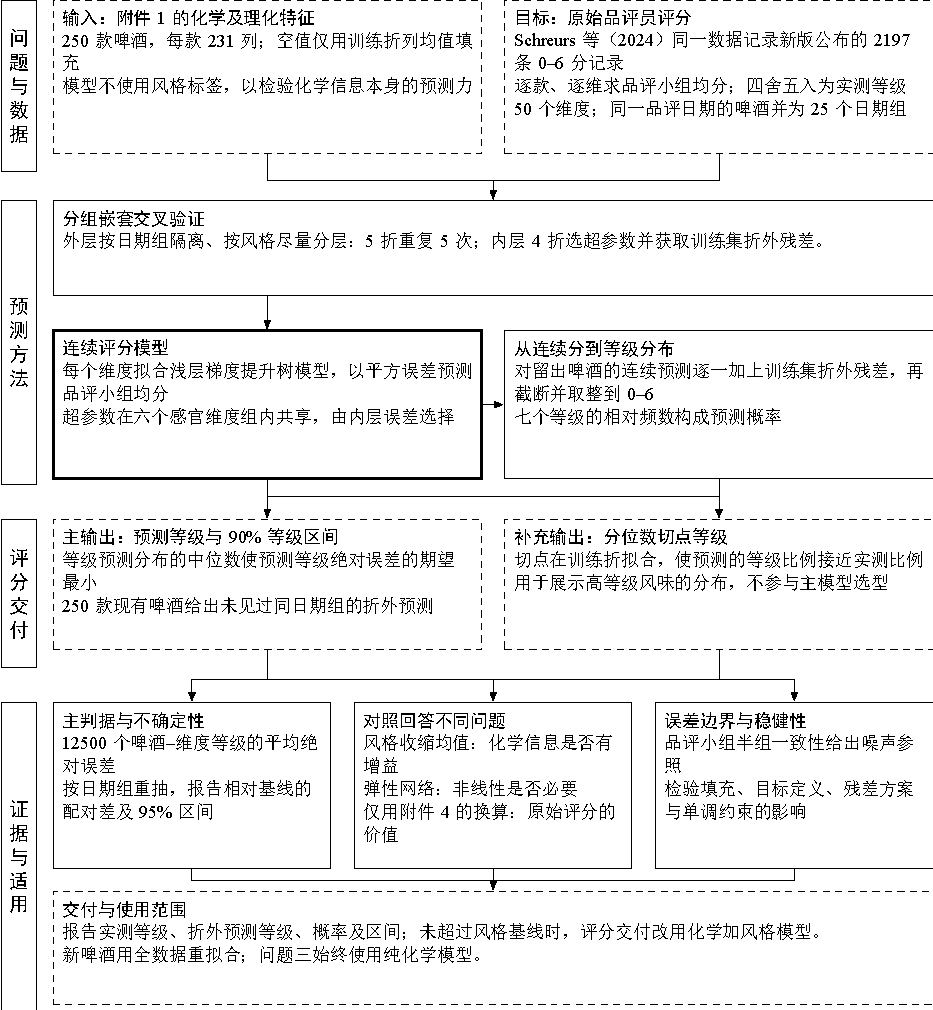
\includegraphics[width=\textwidth]{../figures/q1_methodology_flowchart.pdf}
\caption{问题一方法流程：化学特征与原始评分经日期组嵌套交叉验证得到连续评分与等级预测分布，主输出为分布中位数，第二输出为分位数切点。}
\label{fig:q1-flow}
\end{figure}

对每个感官维度 $d$ 单独训练一个模型 $\hat\mu_{bd}=f_d(X_b)$，以平方损失拟合 $\bar x_{bd}$。
平方损失的最优预测是条件均值，与目标 $\bar x_{bd}$ 的定义一致。
$f_d$ 用 scikit-learn 的 \code{Hist\allowbreak Gradient\allowbreak Boosting\allowbreak Regressor}，是浅层梯度提升树集成。
选用树模型的理由有三点。
第一，Schreurs 等人的论文报告树集成的品评小组测试 $R^2$ 为 0.21 到 0.22，线性回归为 $-4.13$，树集成明显更优。
第二，树只依赖每个特征的顺序，不受 157 个未校准信号列对数底数的影响。
第三，该估计器支持单调约束，也能直接保留缺失值作为敏感性对照。

超参数在每个维度组内共享，以组内平均内层交叉验证的 RMSE 与标准差之比为选择标准。
搜索范围为最大深度 $\{2,3\}$、叶节点最小样本 $\{10,20\}$、学习率 0.05、迭代 $\{100,200,400\}$、$l_2$ 正则 $\{0,1\}$、单调约束开或关。
六个维度组为香气、风味、缺陷、香料啤酒、酸啤酒、基本味口感与总体。
在 250 款啤酒上逐维调参会拟合噪声，因此在 6 个维度组内共享超参数，由内层交叉验证选择。

单调约束来自事先固定的化学知识。
在查看数据之前列出 12 个化合物到感官的配对，其中 11 个符号符合预期，对 6 个直接配对施加约束，包括乙醇到酒精感、苦味单位到苦味、pH 到酸感取负向、乳酸到乳酸感、乙酸到乙酸感、4-乙烯基愈创木酚到酚味。
约束是否开启作为内层交叉验证的超参数，不由外层结果决定。

\subsection{折外残差分布的等级映射与区间估计}

\subsubsection{内层折外残差与等级概率构造}

连续预测需要转为 0 到 6 的等级。
在外层训练集 $\mathcal T$ 上做按日期组分组的 4 折内层交叉验证，得到内层折外预测 $\tilde\mu_{id}$ 与残差 $e_{id}=\bar x_{id}-\tilde\mu_{id}$。
对测试啤酒 $b$，用同一批残差构造预测等级分布：
\begin{equation}\label{eq:q1-p}
\begin{aligned}
p_{bdk}&=\frac{1}{|\mathcal T|}\sum_{i\in\mathcal T}\mathbf 1\!\left\{q(\hat\mu_{bd}+e_{id})=k\right\},\\
F_{bdk}&=\sum_{j\le k}p_{bdj},\qquad k=0,\dots,6 .
\end{aligned}
\end{equation}
式~\eqref{eq:q1-p} 把测试啤酒的预测误差近似为与内层折外残差同分布。
其中 $\mathbf 1\{\cdot\}$ 为指示函数，$p_{bdk}$ 是预测等级为 $k$ 的概率，$F_{bdk}$ 是累积概率。

\subsubsection{分布中位数等级与 90\% 等级区间}

主输出取预测分布的中位数：
\begin{equation}\label{eq:q1-median}
\hat G_{bd}=\min\{k: F_{bdk}\ge 0.5\}.
\end{equation}
主指标是等级 MAE，即平均绝对误差，指预测等级与真实等级之差的绝对值的平均。
在预测分布下使期望等级绝对误差最小的点输出是分布的中位数，因此主输出与主指标匹配。
90\% 等级区间 $[\ell_{bd},u_{bd}]$ 取预测分布的 0.05 与 0.95 分位，$\ell_{bd}=\min\{k:F_{bdk}\ge0.05\}$，$u_{bd}=\min\{k:F_{bdk}\ge0.95\}$。

主输出与四舍五入不同。
零分主导的维度在 0 处截断，残差右偏，等级的中位数不等于 $q(\hat\mu_{bd})$。
完全一致率不作主指标，因为不用化学数据、只输出训练折众数的常数规则完全一致率就有 56.6\%。
主输出、第二输出与主指标都在正式运行前写定。

\subsubsection{分位数切点的补充等级输出}

第二输出取分位数切点，把连续预测 $\hat\mu_{bd}$ 在训练折累积等级频率处的分位数作为切点，输出 $\hat G^{\rm Q}_{bd}=\#\{k:\hat\mu_{bd}\ge c_k\}$，用于保留等级分布的场合。

\subsection{日期组嵌套交叉验证与对照模型设计}

感官评分含品评员之间的系统差异与随机噪声。
同一天品评的啤酒共享出席名单与品评情境，且大多属于同一风格。
随机划分会把同一天品评的啤酒放到训练集与测试集两侧，泄漏同日信息。
因此问题一的交叉验证按日期组隔离，把 37 个品评日期合并成 25 个日期组，每组 5 到 24 款。

表~\ref{tab:q1-setup} 按目标与输入、化学缺失、划分、连续模型、搜索范围、等级与区间、对照与判据七个环节列出正文报告的设置，以及每个设置控制或检验的对象。
软件版本、各折所选参数频数与对照模型的完整搜索网格放附录。

\begin{table}[htbp]
\centering\small
\caption{问题一实验设置与对照}
\label{tab:q1-setup}
\begin{tabular}{p{3.0cm}p{5.4cm}p{4.2cm}}
\toprule
环节 & 正文报告的设置 & 控制或检验什么 \\
\midrule
目标与输入 & 250 款啤酒、231 个化学特征、50 个感官维度；以逐品评员原始评分的每款每维均分为连续目标，均分取整为 0--6 级真值；主模型不输入风格或附件四 & 预测目标、特征与真值同口径 \\
\addlinespace
化学缺失 & 73 个空值在训练折内按列均值填充，测试折不参与预处理 & 填充不泄漏测试信息 \\
\addlinespace
划分 & 37 个日期并为 25 个日期组，按日期组隔离、按风格分层的 5 折 $\times$ 5 次重复，种子 0 到 4，内层同为 4 折 & 同日品评信息不泄漏，调参与报告分开 \\
\addlinespace
连续模型 & 每维一个平方损失 HistGBR，六组内共享超参数，内层按组内平均 RMSE/SD 选参 & 控制模型复杂度 \\
\addlinespace
搜索范围 & 深度 $\{2,3\}$、叶节点 $\{10,20\}$、学习率 0.05、迭代 $\{100,200,400\}$、$l_2$ 正则 $\{0,1\}$、六个单调约束开关由内层选择 & 选参可复现，正文另述迭代下边界检查 \\
\addlinespace
等级与区间 & 内层折外残差构造 0--6 等级概率；分布中位数为主输出，分位数切点为第二输出；90\% 等级区间 & 连续预测转为可交付等级及其不确定性 \\
\addlinespace
对照与判据 & 风格收缩均值为要超越的基线，ElasticNet 检查线性替代，随机森林检查另一种树集成，只用附件四的两阶段方法为对照；主指标等级 MAE，辅助 QWK、完全一致率、$\pm1$ 内比例；按日期组 bootstrap 2,000 次给配对差 95\% 置信区间 & 每个实验为何存在，什么结果支持主张 \\
\bottomrule
\end{tabular}
\end{table}

表~\ref{tab:q1-setup} 的成功标准在运行前声明：主模型等级 MAE 低于风格收缩基线、配对差置信区间上界小于零、且至少 25 个维度逐维 MAE 更低。
指标口径为每次重复合并 250 款折外预测计算，五次再取平均。
最终交付先平均五次概率再取等级，与折外指标口径不同，两者不混用。

\subsection{50 维评分结果、预测误差与区间覆盖}

\subsubsection{整体误差与对照模型比较}

表~\ref{tab:q1-main} 给出主模型与五个关键对照的等级指标。
主模型等级 MAE 为 0.479，风格收缩基线为 0.527，配对差为 $-0.048$，95\% 置信区间为 $[-0.062,-0.034]$，31 个维度逐维 MAE 更低，满足成功标准。

\begin{table}[htbp]
\centering\small
\caption{问题一主结果与关键对照}
\label{tab:q1-main}
\resizebox{\textwidth}{!}{\begin{tabular}{lccccc}
\toprule
模型 & 等级 MAE & 相对主模型的 MAE 差 [95\% CI] & QWK & 完全一致率 & $\pm1$ 内比例 \\
\midrule
风格收缩均值 B1 & 0.527 & $+0.048$ [$0.034$, $0.062$] & 0.095 & 0.559 & 0.931 \\
主模型（化学） & 0.479 & 参照 & 0.290 & 0.581 & 0.950 \\
化学 + 风格 & 0.479 & $-0.0001$ [$-0.0015$, $0.0013$] & 0.289 & 0.580 & 0.950 \\
ElasticNet & 0.481 & $+0.002$ [$-0.010$, $0.013$] & 0.199 & 0.585 & 0.946 \\
随机森林 & 0.472 & $-0.008$ [$-0.015$, $-0.001$] & 0.251 & 0.589 & 0.950 \\
只用附件 C1 & 0.786 & $+0.307$ [$0.271$, $0.341$] & 0.323 & 0.433 & 0.827 \\
\bottomrule
\end{tabular}}
\end{table}

表~\ref{tab:q1-main} 中等级 MAE 为平均绝对误差，QWK 为二次加权 Kappa，完全一致率为预测等级与真实等级相同的单元比例，$\pm1$ 内比例为误差不超过一级的单元比例，单位都是 12,500 个啤酒乘维度单元。

化学加风格一行的结果与主模型相同，回答领域读者最先会问的问题：模型是否只是在识别风格。
只用风格的基线 QWK 为 0.095，在化学特征上再加风格，结果与主模型一致，说明风格信息已由化学谱携带，也支撑问题三只用化学谱给出画像。
随机森林的等级 MAE 为 0.472，低于主模型，但 QWK 为 0.251，低于主模型的 0.290，两者同列呈现，主模型不称各项最优。
只用附件的 C1 按自身规则选定等级映射，端到端等级 MAE 为 0.786，QWK 为 0.323，仍以同一原始等级为真值，其差距主要来自标准化去掉的位置和尺度。

\subsubsection{逐维预测能力与品评信度}

图~\ref{fig:q1-dim} 两栏共用纵轴，50 个维度按六个维度组排列。
左栏为主模型减风格收缩基线的逐维等级 MAE 差，零线区分胜负，标出 31 个胜出维度及各组胜出数。
逐维差只作描述，不把 50 个维度当独立重复求置信区间。
右栏为逐维连续 $R^2$，配同维度的半组信度作短竖线标记。
等级 MAE 受各维度等级分布影响，零分主导的维度 MAE 天然较小，只看左栏会误读维度间差异。
图注写明信度是测量噪声参照，不是严格上限，并注明 $R^2$ 为负的维度。

\begin{figure}[htbp]\centering
\phfig{0.40\textwidth}{左栏为逐维等级 MAE 差（主模型减风格收缩基线），右栏为逐维连续 $R^2$ 与半组信度。}
\caption{逐维增益与可预测性。左栏零线区分主模型与风格收缩基线的逐维胜负，右栏显示逐维连续 $R^2$ 与半组信度。}
\label{fig:q1-dim}
\end{figure}

信度中位数约 0.53，作为噪声参照而非严格性能上限，说明可解释方差的上限就在这一量级。
两半组等级 QWK 为 0.374，是真值本身含抽样噪声的直接证据。
主模型连续 $R^2$ 为 0.184，连续 MAE 为 0.473，连续 Spearman 为 0.360。

\subsubsection{等级分布、高等级收缩与区间覆盖}

表~\ref{tab:q1-rules} 比较四种等级规则。
预测分布中位数与四舍五入的等级 MAE 分别为 0.479 与 0.490，中位数更低且不增加参数。
分位数切点的等级 MAE 为 0.578，高于中位数，但 QWK 为 0.371，高于中位数的 0.290，预测 5 到 6 级的占比为 1.57\%，接近真值的 0.968\%。
主输出服务单款误差最小化，第二输出服务等级分布描述，两者同时交付。

\begin{table}[htbp]
\centering\small
\caption{问题一等级规则比较}
\label{tab:q1-rules}
\resizebox{\textwidth}{!}{\begin{tabular}{lcccc}
\toprule
规则 & 等级 MAE & QWK & 完全一致率 & 预测 5--6 级占比 \\
\midrule
常数等级（训练折众数） & 0.549 & $-0.006$ & 0.566 & 0\% \\
四舍五入 & 0.490 & 0.293 & 0.565 & 0.04\% \\
预测分布中位数（主输出） & 0.479 & 0.290 & 0.581 & 0.02\% \\
分位数切点（第二输出） & 0.578 & 0.371 & 0.531 & 1.57\% \\
\bottomrule
\end{tabular}}
\end{table}

保持等级分布提高 QWK，但单款啤酒的误差变大。
原因是模型只解释了一部分方差，最优的单点预测必然向中间收缩。
要让等级分布与真值一致，就得把部分啤酒推离它最可能的等级。
这一取舍由表~\ref{tab:q1-rules} 与图~\ref{fig:q1-grade} 共同呈现。

图~\ref{fig:q1-grade} 左栏为真值、主输出、第二输出的 0 到 6 级频率，右栏为按真实等级分层的主输出召回率。
$\pm1$ 内比例约 95\% 会掩盖高等级漏判，本图回答这一疑虑。
主输出几乎不给出 5 到 6 级，5 级真值 112 个单元、6 级 9 个单元的召回率接近零，误差集中在相邻等级。
第二输出给出 1.57\% 的 5 到 6 级，更接近真值。

\begin{figure}[htbp]\centering
\phfig{0.40\textwidth}{左栏为真值、主输出、第二输出的 0--6 级频率，右栏为按真实等级分层的主输出召回率。}
\caption{误差集中的等级。左栏显示三种等级频率，右栏显示主输出按真实等级分层的召回率，图注注明每栏分母。}
\label{fig:q1-grade}
\end{figure}

90\% 等级区间覆盖 97.2\%，平均宽度 1.97 级，略宽于名义值，来自等级的离散性与折外残差的保守性。

\subsubsection{交付评分示例}

赛题要求给出评分结果，表~\ref{tab:q1-delivery} 展示交付物本身。
选款规则事先固定，在 Pils/Lager、Tripel、Kriek 三个风格中各取原始评分记录数最多的一款，与问题三的风格相连。
行为 15 个属性，列为三款啤酒的 Aroma 与 Flavour，共 6 列。
单元格写交付等级与 90\% 区间，再附实测等级。
全部 250 款作为机器可读补充文件交付。

\begin{table}[htbp]
\centering\small
\caption{交付评分示例：三款啤酒的 15 个属性}
\label{tab:q1-delivery}
\resizebox{\textwidth}{!}{\begin{tabular}{lcccccc}
\toprule
属性 & \multicolumn{2}{c}{Pils/Lager} & \multicolumn{2}{c}{Tripel} & \multicolumn{2}{c}{Kriek} \\
 & Aroma & Flavour & Aroma & Flavour & Aroma & Flavour \\
\midrule
malt\_all & \ph & \ph & \ph & \ph & \ph & \ph \\
\addlinespace
\multicolumn{7}{l}{\small 单元格格式为交付等级 [90\% 区间] / 实测等级，取自最终交付口径 $G_{hat}$，与折外指标口径不同。} \\
\addlinespace
\multicolumn{7}{l}{\small 占位单元格由 Coding 从 \code{q1\_final\_scores.csv} 导出，三款啤酒按选款规则在三个风格中取评分记录数最多者。} \\
\bottomrule
\end{tabular}}
\end{table}

\subsection{缺失值处理、评分目标与等级规则的敏感性分析}

敏感性分析共八项，其中七项的等级 MAE 配对差置信区间含 0，交付等级变化不超过 5.2\%。
训练目标改为训练折内估计的啤酒效应、化学缺失的三种替代填充、barnyard 的排除、四个综合指标的删除、附件八冲突单元替换、单调约束全开或全关，都不改变主要结论。
网格扩展检查在重复 0 上把迭代下界扩展到 10 到 200，外层连续 MAE 与 $R^2$ 不变，Spearman 低 0.019，未改善外层预测，主网格保持不变。
只用附件的对照 C1，其零点还原的中间结果见表~\ref{tab:prep-reference}，端到端结果见表~\ref{tab:q1-main}。

\section{问题二：基于共表达图的关键化合物识别}

问题二利用附件二的化合物相关矩阵构建共表达图，结合附件一的化学特征，给出每个感官维度上关联最强的三个化合物。
估计目标 $T_d=(t_{d1},t_{d2},t_{d3})$ 定义为在 250 款啤酒上按控制已选化合物后的秩关联依次最强、且两两不属于同一共表达模块的 3 个化合物。
这是关联定义，不是因果定义。

题目要求找出关键化合物，本章将其操作化为关联结果。
附件中没有干预数据，不能直接推断因果，化学合理性在结果产生后给出机理解释。
唯一独立于这 250 款啤酒的核验是作者发布的加标实验，其结论只在第~\ref{subsec:spike} 节报告。
因此本章的核心是让关联结果可重复、可独立于感官数据检验，而不是宣称因果。

\subsection{基于斯皮尔曼相关的共表达图与平均连接层次聚类}

候选化合物为附件一的 231 列减去 5 个综合指标和 1 个内标，共 225 个。
综合指标 $esters\_sum$、$aroma\_hops\_sum$、$acids\_sum$、$sulfur\_sum$、$kcalperc$ 由其他化合物计算得到，各自几乎是某一个组成成分的副本，与其对应成分的 Spearman 相关系数绝对值分别为 0.92、0.96、0.97、0.78、0.85。
把它们列为候选会使同一信息以总量和成分两次入选，且题目要求的是化合物。
内标 3-甲基-2-丁烯醛在附件八中被标为内标溶液，反映测量过程，不反映啤酒组成。
6 个排除列仍作为图的注释节点保留，用于展示综合指标与成分的关系。

图~\ref{fig:q2-flow} 给出问题二的完整流程。
化合物与感官秩经共表达图、模拟还原支持的图约束前向选择与置换检验，再经日期组重抽和替代方法，得到化学证据与前三项关联候选。

\begin{figure}[htbp]\centering
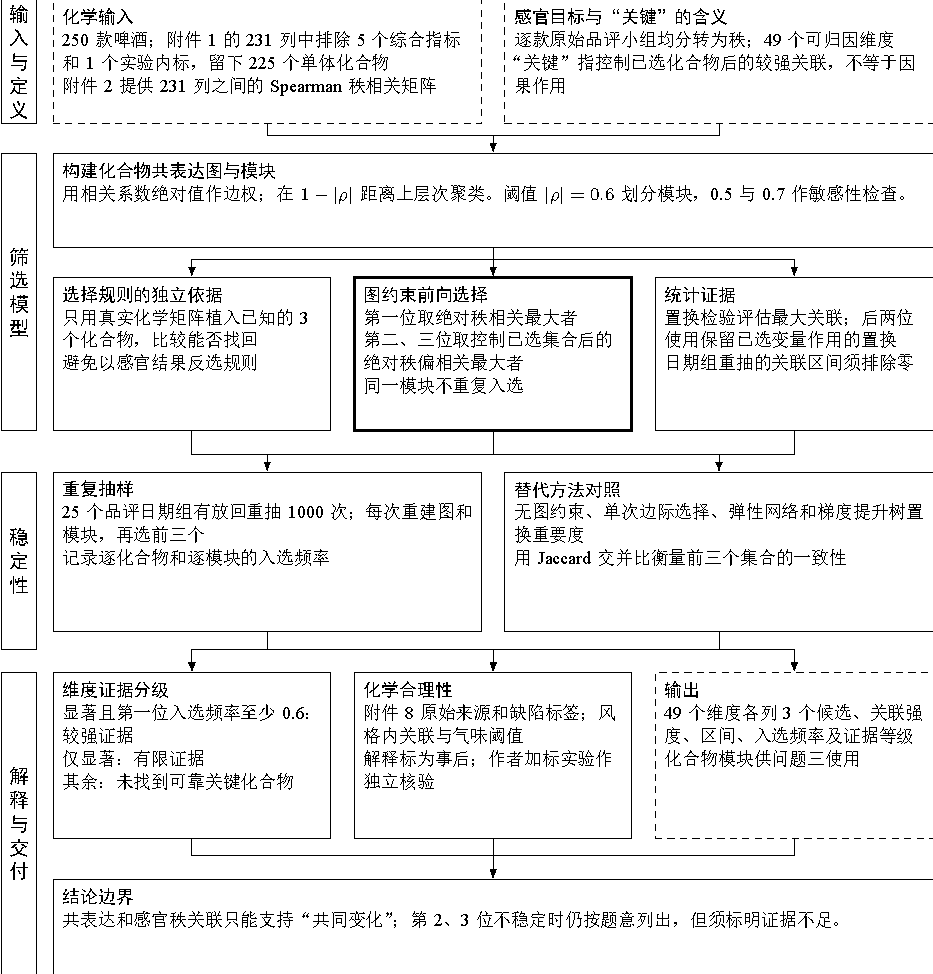
\includegraphics[width=\textwidth]{../figures/q2_methodology_flowchart.pdf}
\caption{问题二方法流程：化合物与感官秩经共表达图、图约束前向选择与置换检验得到关键化合物，稳定性由日期组重抽量化。}
\label{fig:q2-flow}
\end{figure}

共表达图 $G_\tau$ 的节点为 231 列，边权为两两 Spearman 系数的绝对值 $\lvert\rho_{jk}\rvert$，符号作为边属性保留。
使用无符号权重是因为强相关几乎都是正相关，$\lvert\rho\rvert\ge0.5$ 的 597 条边中只有 13 条为负。
模块由 $1-\lvert\rho\rvert$ 上的平均连接层次聚类得到，在高度 $1-\tau$ 处切开。
平均连接只在两组之间平均边权不低于 $\tau$ 时合并，因此每个模块内的化合物彼此平均相关至少约为 $\tau$。

主值 $\tau=0.6$，其依据有三点。
第一，0.6 是候选间 Spearman 相关系数绝对值的 99\% 分位，仅最强的 1\% 化合物对的相关达到该阈值。
第二，$\tau=0.5$ 时模块混入不同来源的化合物，来源纯度（多成员模块中占多数的附件八来源类别所占比例的平均值）降至 0.70，划分可重复性（调整兰德指数 ARI）降至 0.66。
第三，$\tau=0.7$ 时只有 65 个化合物属于多成员模块，冗余控制覆盖的范围变小。
主值下得到 161 个模块，其中 33 个多成员模块覆盖 97 个化合物，代表性模块包括乙醇、乙酸乙酯、己酸乙酯、甘油构成的发酵强度模块，以及辛酸乙酯、癸酸乙酯构成的中链脂肪酸乙酯模块。
化合物层的入选频率在三个 $\tau$ 下相同，所以 $\tau$ 主要影响模块层的解读。

\subsection{共表达模块约束下的秩偏相关前向选择}

第 1 位取边际关联最强者：
\begin{equation}\label{eq:q2-top1}
t_{d1}=\arg\max_{j\in\mathcal C}\,\lvert r_{jd}\rvert .
\end{equation}
其中 $\mathcal C$ 为 225 个候选化合物集合，$r_{jd}$ 是化合物 $j$ 与维度 $d$ 的 Spearman 系数，在两者的标准化秩上计算。
第 $k$ 位（$k=2,3$）在控制已选集合 $S$ 后取秩偏相关最强者。
令 $H_S$ 为向 $\{\mathbf 1,\tilde x_s:s\in S\}$ 张成空间的投影，
\begin{equation}\label{eq:q2-partial}
\begin{aligned}
e_y&=(I-H_S)\tilde y_d,\qquad e_j=(I-H_S)\tilde x_j,\\
r_{jd\mid S}&=\frac{e_j^\top e_y}{\lVert e_j\rVert\,\lVert e_y\rVert},\qquad
t_{dk}=\arg\max_{j\in\mathcal C,\ M(j)\notin M(S)}\,\lvert r_{jd\mid S}\rvert .
\end{aligned}
\end{equation}
式~\eqref{eq:q2-partial} 中 $r_{jd\mid S}$ 是秩上的偏相关，衡量化合物 $j$ 在已选化合物之外还能解释多少维度排序。
图在第一处排除与已选者属于同一模块的化合物，在第二处把同模块化合物与入选者一起报告。

\subsection{模拟实验验证、置换检验与日期组重抽样}

选用前向选择而不用边际选择，由模拟还原实验决定。
边际选择按 $\lvert r_{jd}\rvert$ 降序、每模块至多一个取前 3，会反复选入第 1 个植入化合物的间接相关者。
在真实化学矩阵上随机植入 3 个来自不同模块的化合物，按秩线性组合加噪声生成维度，第 1 个植入化合物的 $r$ 取 0.2、0.3、0.45，权重取 (1, 0.75, 0.5) 与 (1, 1, 1)，每种设置 1,000 次。
前向选择在 $r\ge0.3$ 时找回率更高，其中找回率指植入化合物被选入前 3 位的比例，而观测数据中 49 个维度第 1 位关键化合物的 $\lvert r\rvert$ 中位数为 0.38，四分位为 0.30 到 0.48，处于前向选择占优的区间。
模拟只用化学矩阵，不使用感官数据，因此这一选择没有利用观测到的 Top-3 内容。

图~\ref{fig:q2-recovery} 为 2 乘 3 小多图，行为两种植入权重，列为植入名次 1 到 3。
横轴为第 1 个植入化合物的 $r$，纵轴为化合物层找回率，两条线为前向选择与图约束边际选择。
每格加竖向阴影带，表示 49 维 Top-1 相关绝对值的四分位范围及中位线。
图注写明每格 1,000 次，二项 95\% 区间约正负 0.03，不画误差线。
前向选择在中等与较大效应量下找回率更高，在小效应量下与边际选择相当，两种规则的实际差异按本图呈现。

\begin{figure}[htbp]\centering
\phfig{0.38\textwidth}{2 乘 3 找回率小多图，行为两种权重，列为植入名次 1 到 3，横轴为第 1 个植入化合物的 $r$，纵轴为化合物层找回率。}
\caption{规则依据实验的找回率。两条线为前向选择与图约束边际选择，竖向阴影带为观测 Top-1 相关的四分位范围。}
\label{fig:q2-recovery}
\end{figure}

每个维度的显著性门槛由置换检验给出。
打乱 $\tilde y_d$ 的行 1,000 次，取 225 个化合物边际相关绝对值的最大值，得到维度 $d$ 的零分布，95\% 分位记为 $q_d$。
第 2、3 位用 Freedman--Lane 置换，打乱 $e_y$ 后在可选化合物上取偏相关绝对值的最大值。
逐行打乱忽略日期组内的相关，零分布偏窄，因此每个入选项另外用日期组簇 bootstrap 计算 95\% 置信区间。
入选项同时满足得分超过门槛与置信区间不含 0 时记为显著。

稳定性重抽以日期组为单位，而不是以单款啤酒为单位。
同一天品评的啤酒共享出席名单和品评情境，且大多属于同一风格。
按单款啤酒重抽会把这些相关性当作独立样本，高估有效样本量。
25 个日期组是可直接观测、粒度更粗的分组，重抽时每次抽取 25 个日期组并拼接其中的啤酒。

表~\ref{tab:q2-setup} 按输入与目标、缺失与秩、图与模块、选择规则、显著性、稳定性、规则依据实验、对照方法八个环节列出正文报告的设置。

\begin{table}[htbp]
\centering\small
\caption{问题二实验设置与对照}
\label{tab:q2-setup}
\begin{tabular}{>{\raggedright\arraybackslash}p{3.0cm}>{\raggedright\arraybackslash}p{5.4cm}>{\raggedright\arraybackslash}p{4.2cm}}
\toprule
环节 & 正文报告的设置 & 控制或检验什么 \\
\midrule
输入与目标 & 250 款啤酒；附件一 231 列剔除 5 个综合指标与内标，剩 225 个候选；49 个维度，barnyard 记作同 stale\_hops；感官目标为原始评分均分的秩 & 候选都是化合物或理化指标，目标与问题一同口径 \\
\addlinespace
缺失与秩 & 8 个单化合物列共 60 个空值按列均值填充，每次 bootstrap 样本内重算；信号下限按并列最低秩处理 & 填充值不解释为浓度 \\
\addlinespace
图与模块 & 边权取 $\lvert\rho\rvert$，$1-\lvert\rho\rvert$ 上平均连接层次聚类，$\tau=0.6$ 切割 & 模块内平均相关至少约为 $\tau$ \\
\addlinespace
选择规则 & 第 1 位取最大 $\lvert r_{jd}\rvert$，第 2、3 位取控制已选集合后的秩偏相关最大者，同一模块至多入选 1 个 & 用条件关联去除间接相关者 \\
\addlinespace
显著性 & 置换 1,000 次，第 1 位用全体候选最大相关零分布的 95\% 分位，第 2、3 位用 Freedman--Lane 置换，并同时要求日期组 bootstrap 95\% 置信区间不含 0 & 维度内多重比较与日期组内相关 \\
\addlinespace
稳定性 & 25 个日期组有放回重抽 $B=1000$，每次重建相关矩阵与模块，报告化合物层与模块层入选频率 $\pi^c$、$\pi^m$，分档界限 0.6 与 $1/3$ & 结论对样本扰动的稳定程度 \\
\addlinespace
规则依据实验 & 真实化学矩阵植入 3 个不同模块的化合物，权重 (1,0.75,0.5) 与 (1,1,1)，第 1 个植入化合物的 $r$ 取 0.2、0.3、0.45，每种设置 1,000 次，噪声含日期组偏移 & 只用化学矩阵、不用感官数据，回应根据结果改规则的质疑 \\
\addlinespace
对照方法 & 无图约束边际选择、图约束边际选择、ElasticNet、问题一梯度提升树、风格内分析 & 每种对照对应方法的一处改动 \\
\bottomrule
\end{tabular}
\end{table}

Top-3 是关联而非因果。
维度等级按 Top-1 的显著性与入选频率分为三档，A 级为 Top-1 显著且 $\pi^c\ge0.6$，B 级为 Top-1 显著但不满足 A，C 级为 Top-1 不显著。
选择规则在预运行后由边际选择改为前向选择，已在正文披露。

\subsection{各感官维度的前三项关键化合物与稳定性结果}

\subsubsection{前三项结果与关联方向}

表~\ref{tab:q2-rep} 给出代表维度的 Top-3 证据。
代表维度按事先规则选取，每个维度组至少一个，优先与加标属性对应的维度，含一个 C 级维度，共 21 行。
化学解释写在正文，不入表。
选择得分、95\% 置信区间与风格内系数从最终合理性表导出，完整 147 项按六个维度组放附录。

\begin{table}[htbp]
\centering\small
\caption{代表维度的 Top-3 证据}
\label{tab:q2-rep}
\begin{tabular}{lclclcl}
\toprule
维度（等级） & 名次 & 化合物 & 方向 & $\pi^c$ & OAV$\ge$1 占比 \\
\midrule
A\_esters\_all（A） & 1 & 己醇 & $+$ & 0.61 & 无阈值 \\
 & 2 & 乳酸 & $+$ & 0.36 & 0.17 \\
 & 3 & 乙醛 & $+$ & 0.33 & 0.00 \\
\addlinespace
F\_malt\_all（A） & 1 & pH & $+$ & 0.79 & 无阈值 \\
 & 2 & 乙醇 & $+$ & 0.47 & 0.98 \\
 & 3 & 色度 & $+$ & 0.47 & 无阈值 \\
\addlinespace
bitternes（A） & 1 & 苦味单位 & $+$ & 1.00 & 0.86 \\
 & 2 & 辛酸乙酯 & $+$ & 0.74 & 0.26 \\
 & 3 & 铁 & $-$ & 0.09 & 0.48 \\
\addlinespace
body（A） & 1 & 乙醇 & $+$ & 0.99 & 0.98 \\
 & 2 & 色度 & $+$ & 0.56 & 无阈值 \\
 & 3 & 铁 & $-$ & 0.04 & 0.48 \\
\addlinespace
lactic（A） & 1 & pH & $-$ & 0.95 & 无阈值 \\
 & 2 & 乙酸异戊酯 & $-$ & 0.88 & 0.84 \\
 & 3 & 蛋白质 & $+$ & 0.53 & 1.00 \\
\addlinespace
clove（A） & 1 & 柠檬烯 & $+$ & 0.80 & 无阈值 \\
 & 2 & $\alpha$-卡拉烯 & $-$ & 0.21 & 无阈值 \\
 & 3 & 乙酸丙酯 & $+$ & 0.20 & 无阈值 \\
\addlinespace
t2n（C） & 1 & $\beta$-水芹烯 & $-$ & 0.23 & 无阈值 \\
 & 2 & 辛酸乙烯酯 & $+$ & 0.18 & 无阈值 \\
 & 3 & 己醇 & $-$ & 0.04 & 无阈值 \\
\bottomrule
\end{tabular}
\end{table}

\subsubsection{化合物及模块入选频率}

图~\ref{fig:q2-network} 重绘共表达网络，只画多成员模块的化合物和 6 个注释节点，单成员节点只在图注计数。
节点颜色为附件八来源，大小为该化合物进入主方法 Top-3 的维度数，未入选者空心。
边宽与 $\lvert\rho\rvert$ 成正比，负相关边虚线。
标注至少 3 个成员模块的枢纽、全部入选化合物，以及发酵强度、中链脂肪酸乙酯等代表模块。

\begin{figure}[htbp]\centering
\phfig{0.40\textwidth}{共表达网络，节点按附件八来源着色、按入选维度数定大小，模块内力导向排布，边宽与相关绝对值成正比。}
\caption{化合物共表达网络。只画多成员模块与注释节点，图注计数单成员节点并说明综合指标的排除理由。}
\label{fig:q2-network}
\end{figure}

图~\ref{fig:q2-stability} 左栏为 49 行乘 3 名次的化合物层入选频率 $\pi^c$ 热图，行按六个维度组分块，三档离散色阶，格内写两位小数，不显著项加斜线纹。
右栏为名次 1 到 3 各一根堆叠柱，按稳定、中等、不稳定的维度数堆叠，叠加化合物层与模块层入选频率的均值标记，两者之差反映同模块轮换。
入选频率按名次为 0.60、0.36、0.22，稳定、中等、不稳定项分别为 33、41、73。
此图支持多数维度可靠支持的关键化合物为 1 到 2 个这一结论。

\begin{figure}[htbp]\centering
\phfig{0.44\textwidth}{左栏为 49 行乘 3 名次的入选频率热图，行按六个维度组分块；右栏为三个名次各一根堆叠柱。}
\caption{关键化合物的稳定性。左栏为逐维入选频率热图，右栏为三个名次按稳定程度堆叠的维度数。}
\label{fig:q2-stability}
\end{figure}

\subsubsection{证据分级与支持不足的维度}

图~\ref{fig:q2-jaccard} 为竖向柱状图，横轴为五个方法，纵轴为 49 维平均 Jaccard，每个方法画化合物层、模块层两根柱，柱顶标 Top-1 一致比例。
Jaccard 系数为两个集合交集与并集大小之比，衡量两个方法选出化合物的重合程度。
随机 3 元集合基线 0.008 画细虚线，说明重合不是偶然。
主方法与无图约束边际选择、图约束边际选择的化合物层 Jaccard 分别为 0.339 与 0.382，Top-1 按构造相同。
与 ElasticNet 为 0.573，与梯度提升树为 0.267，与风格内分析为 0.259。
梯度提升树的 Top-1 一致比例只有 0.45，解释为估计对象不同，相关特征下置换重要度被稀释，不同的维度在附录并列给出。

\begin{figure}[htbp]\centering
\phfig{0.29\textwidth}{方法间 Jaccard 柱状图，横轴为五个方法，纵轴为 49 维平均 Jaccard，每个方法画化合物层、模块层两根柱。}
\caption{方法间 Jaccard。细虚线为随机 3 元集合基线，柱顶标注 Top-1 一致比例。}
\label{fig:q2-jaccard}
\end{figure}

显著性门槛 $q_d$ 的中位数为 0.229，第 1、2、3 位超过门槛的维度分别为 48、39、21 个。
维度等级为 A 级 26 个、B 级 22 个、C 级 1 个，C 级为 t2n。
共变标记项数 88 个，模块不可分假设被推翻 0 项。
附件二与附件六的复算误差分别为 $2.05\times10^{-15}$ 与 $6.66\times10^{-16}$，说明列对齐与逐对删除的实现正确。
C 级维度 t2n 的零膨胀检查未发现关联随零膨胀而增强的证据。

\subsection{来源标签、气味活度值与混合物加标的化学合理性论证}

\subsubsection{来源、缺陷标签与气味活度值证据}

以苦味为例，苦味单位的入选频率为 1.00，与苦味的关联方向为正，气味活度值超过 1 的啤酒占 86\%。
以乳酸为例，pH 与乳酸感的关联方向为负，说明酸度由 pH 直接刻画。
以 t2n 为例，其 Top-1 不显著，标记为未找到可靠的关键化合物，Top-3 仍列出供参考。

\subsubsection{风格内关联与共变化合物解释}

图~\ref{fig:q2-scatter} 为 147 个点的散点图，横轴为合并边际 Spearman $r_{jd}$，纵轴为风格内 $r^{(s)}_{jd}$，点形状表示名次，颜色表示风格内置信区间是否含 0。
主 Top-3 的 147 项中 98\% 在风格内保持同号，风格内与合并系数之比的中位数为 0.66。
有 18 项的风格内 $\lvert r^{(s)}\rvert<0.1$，即其关联几乎完全来自风格之间，包括乳酸到乳酸感、pH 到酸感、乙醇到麦芽风味。

\begin{figure}[htbp]\centering
\phfig{0.38\textwidth}{合并边际相关对风格内相关的散点，147 个点，标出乳酸到乳酸感、pH 到酸感、乙醇到麦芽风味。}
\caption{合并与风格内关联。参考线为 $y=x$ 与 $y=0$，颜色表示风格内置信区间是否含 0。}
\label{fig:q2-scatter}
\end{figure}

\subsubsection{独立混合物加标实验的对应与解释}
\label{subsec:spike}

表~\ref{tab:q2-spike} 为作者加标实验的同人配对差，加标物为 6 到 7 种化合物的混合物。
酯类加标在三组中都提高 Esters，支持酯类作为酯类维度的关键因素。
未加入任何酒花化合物，Hops 与 Bitterness 不变，是一组阴性对照。
Fullness 在三组中都提高，与 body 的 Top-1 乙醇及其同模块的甘油方向一致，但无乙醇组同样提高，说明甘油或其他成分足以产生该效应。

\begin{table}[htbp]
\centering\small
\caption{加标实验的同人配对差与对应维度}
\label{tab:q2-spike}
\resizebox{0.9\textwidth}{!}{\begin{tabular}{lcccl}
\toprule
属性 & Blond 含乙醇 $n{=}20$ & Blond 无乙醇 $n{=}13$ & NABLAB 无乙醇 $n{=}13$ & 对应维度（Top-1） \\
\midrule
Esters & 0.90（4.7） & 1.08（2.9） & 1.31（5.0） & 酯类（己醇 / 蛋白质） \\
Fullness & 1.30（6.3） & 1.31（3.0） & 1.38（4.8） & body（乙醇） \\
Alcohol warming & 1.10（4.2） & 0.92（4.4） & 0.08（0.6） & alcohol（乙醇） \\
Sweetness & 1.15（4.4） & 0.69（2.0） & 1.00（3.1） & sweetness（癸酸乙酯） \\
Hops & $-0.15$（$-0.5$） & 0.00（0.0） & $-0.08$（$-0.2$） & 酒花（辛酸乙酯 / 苦味单位） \\
Bitterness & 0.05（0.2） & $-0.15$（$-0.6$） & $-0.31$（$-0.9$） & bitternes（苦味单位） \\
Malt & 0.45（2.0） & $-0.23$（$-1.0$） & 0.00（0.0） & 麦芽（色度 / pH） \\
Overall & 1.05（2.8） & 1.15（3.6） & 1.08（3.5） & overall（乙酸乙酯） \\
\bottomrule
\end{tabular}}
\end{table}

\subsection{模块阈值、候选集合与感官目标的敏感性分析}

敏感性分析的主要结论是结论对模块阈值、候选集合、缺失处理与附件取值稳定，唯一的例外是感官目标改用附件四的标准化值后 Top-3 与等级变化较大，结论以原始评分均值为准。

\section{问题三：风格条件生成、感官画像与跨风格迁移}

问题三以细分风格标签为条件学习生成模型，在给定风格下生成化合物谱并给出感官画像，再把一种风格的化合物谱迁移为另一种风格，且缺陷化合物不恶化。
估计目标有三项：风格条件分布 $p(x\mid s)$、感官画像、以及满足两层缺陷约束的迁移映射。

\subsection{秩变换与风格条件潜在高斯模型}

图~\ref{fig:q3-flow} 给出问题三的完整流程。
风格和化学谱经秩变换与风格条件潜在高斯模型，经留出啤酒的保真、新颖性、可用性检查，得到感官画像与风味指纹，再经潜空间平移、化学投影、感官路径与原尺度复查完成迁移。

\begin{figure}[H]\centering
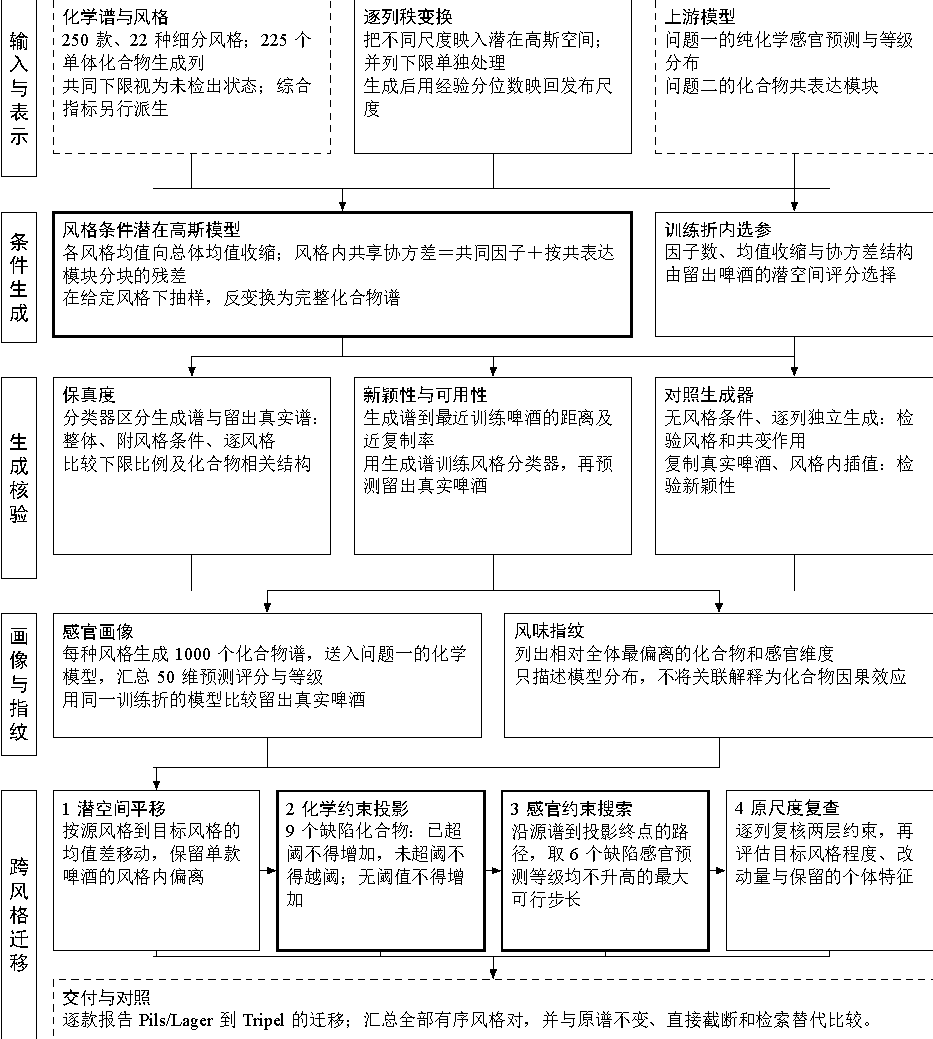
\includegraphics[width=\textwidth]{../figures/q3_methodology_flowchart.pdf}
\caption{问题三方法流程：风格和化学谱经秩变换与风格条件潜在高斯模型生成化合物谱，迁移经潜空间平移、化学投影、感官路径与原尺度复查。}
\label{fig:q3-flow}
\end{figure}

\subsubsection{并列下限的秩正态变换与经验分位数反变换}

生成器在逐列秩变换后的潜变量上建模。
对列 $j$ 取训练折的非缺失观测，把相同取值合并为块，块 $k$ 覆盖经验累积概率区间 $(l_k,h_k]$，块内所有观测的潜变量取标准正态在该区间上的条件期望：
\begin{equation}\label{eq:q3-rank}
\phi_j(x)=\mathbb E\!\left[Z\mid \Phi^{-1}(l_k)<Z\le\Phi^{-1}(h_k)\right]=\frac{\varphi(\Phi^{-1}(l_k))-\varphi(\Phi^{-1}(h_k))}{h_k-l_k} .
\end{equation}
式~\eqref{eq:q3-rank} 中 $\varphi$ 与 $\Phi$ 分别是标准正态的密度与分布函数。
无并列的取值时该式近似于正态得分，下限块的潜变量是截断正态的均值。
反变换 $x_j=Q_j(\Phi(u_j))$ 中 $Q_j$ 是保留并列取值全部概率质量的逆经验分布函数，把下限的整个概率区间映回下限值。

\subsubsection{风格均值收缩与因子模型加模块分块残差的协方差估计}

在潜空间中，同一风格内的潜变量服从多元正态分布：
\begin{equation}\label{eq:q3-gauss}
u_b\mid s(b)=s\ \sim\ \mathcal N(\mu_s,\ \Sigma_W),\qquad \Sigma_W=\Lambda\Lambda^\top+\Psi_M .
\end{equation}
式~\eqref{eq:q3-gauss} 中 $u_b$ 为啤酒 $b$ 的潜变量向量，$k$ 为因子数，$\Lambda$ 为 $225\times k$ 的因子载荷，$\Psi_M$ 为按问题二共表达模块分块的特异协方差。
风格均值向全局均值收缩：
\begin{equation}\label{eq:q3-shrink}
\hat\mu_s=\frac{n_s\bar u_s+\kappa\,\bar u}{n_s+\kappa},
\end{equation}
式~\eqref{eq:q3-shrink} 中 $n_s$ 为风格 $s$ 的啤酒数，$\bar u_s$ 为风格 $s$ 的样本均值，$\bar u$ 为全局均值，$\kappa$ 为收缩强度。
该式与问题一基线的收缩形式相同，小样本风格的均值估计由收缩稳定。
风格内协方差由合并风格内残差估计，先拟合因子载荷，再保留同一模块内的元素与对角元作为 $\Psi_M$，负特征值截到 $10^{-3}$ 保证正定。
各风格共享同一个 $\Sigma_W$，因为单个风格最多 31 款、少于 225 维，风格专属的完整协方差不可估计。

风格只解释每个化合物潜变量方差的一部分，风格解释的潜变量方差比例 $\eta^2$ 的中位数为 0.250，因此生成器必须同时刻画风格均值和风格内变化，只生成风格均值会丢掉约四分之三的方差。
风格内变化有低维结构，合并风格内残差的前 30 个主成分解释 72\% 的方差。
纯因子模型会衰减强相关的化合物对，模块块恢复这一共变，预运行中留出真实啤酒的模块内平均 Spearman 为 0.724，加模块块后生成样本为 0.680。

\subsection{生成模型选参与留出验证设计}

对生成结果提出三层合理性要求。取值层要求每列取值落在 250 款啤酒的观测范围内，未检出的下限作为离散状态按应有比例出现，综合指标与其成分一致。
分布层要求风格 $s$ 的生成样本与留出的风格 $s$ 真实啤酒在带风格标签的分类器双样本检验（C2ST，AUC 接近 0.5 表示未发现可区分性）中未表现出明显可区分性，也被独立的风格判别器判为 $s$。
新颖性要求生成样本不是训练啤酒的复制品。

生成器按风格分层、以单款啤酒为单位的 5 折交叉验证重复 5 次，种子 0 到 4；涉及感官标签的画像另用问题一的日期组外层划分，避免同一品评日期进入训练集与留出集两侧。
判别器与分类检验用随机森林 500 棵树、只用真实啤酒训练，与生成器不共享高斯假设；分类检验的置换 200 次并做真实对真实参照。
对照生成器五个：纯因子去掉模块块，无风格去掉风格条件，逐列独立去掉化合物间共变，复制直接复用训练啤酒，风格内插值在潜空间插值。
完整实验设置表与参数网格进附录。

选参在外层训练集内按留出潜空间评分完成，25 个外层折中有 24 折选因子加模块块、因子数 10、收缩强度 2，1 折选收缩强度 5；交付的全数据模型按同一规则选因子数 15、收缩强度 5。
下文的结果均以外层留出啤酒评价，选参不与报告复用同一划分。

\subsection{生成化合物谱及保真度、新颖性与可用性结果}

表~\ref{tab:q3-gen} 报告生成器验证的主要检验、对照与参照。
主模型在验收项 (a) 未通过：区分留出真实啤酒与生成样本的两样本分类检验，合并曲线下面积（AUC）为 0.589，条件曲线下面积为 0.576，均超出 $|\mathrm{AUC}-0.5|\le0.05$ 的预设标准，置换检验 $p$ 值为 0.017 与 0.032，真实对真实参照为 0.494 与 0.501，无风格对照为 0.642 与 0.634，逐列独立对照为 0.668，说明生成样本与真实啤酒仍可被区分，且这一差异来自下限状态共现而非检验偏差。
其余 (b) 到 (e) 通过：最近邻距离比 1.111，近复制率 0；在生成样本上训练的风格判别器识别留出真实啤酒的准确率为 0.481，真实对真实为 0.550；下限比例误差 0.021，复制参照为 0.014；模块内平均相关 0.667，真实留出为 0.724。
事后诊断把差异主要归于下限状态的共现：只用下限指示的分类检验 AUC 为 0.646，高于全谱的 0.564，生成样本中不同列同时未检出的程度约为真实的一半；其次是生成离散偏小，离散比为 1.17；把真实值截到训练范围后 AUC 不变，排除越界取值这一原因。

\begin{table}[H]
\centering\small
\caption{问题三生成器验证（占位，正式产物验收后填写）}
\label{tab:q3-gen}
\begin{tabular}{lcccccc}
\toprule
指标 & 主模型 & 纯因子 & 无风格 & 逐列独立 & 真实留出参照 & 验收阈值 \\
\midrule
取值层：下限比例误差 & 占位 & 占位 & 占位 & 占位 & 占位 & 占位 \\
取值层：每款下限列数 & 占位 & 占位 & 占位 & 占位 & 占位 & 占位 \\
分布层：合并 C2ST AUC & 占位 & 占位 & 占位 & 占位 & 占位 & 占位 \\
分布层：条件 C2ST AUC & 占位 & 占位 & 占位 & 占位 & 占位 & 占位 \\
分布层：风格内相关误差 & 占位 & 占位 & 占位 & 占位 & 占位 & 占位 \\
分布层：模块内相关 & 占位 & 占位 & 占位 & 占位 & 占位 & 占位 \\
新颖性：判别器距离比 & 占位 & 占位 & 占位 & 占位 & 占位 & 占位 \\
新颖性：近复制率 & 占位 & 占位 & 占位 & 占位 & 占位 & 占位 \\
\bottomrule
\end{tabular}
\end{table}

\subsection{基于评分预测分布的感官画像与风味指纹}

\subsubsection{生成谱的 50 维感官画像与留出参照}

感官画像由问题一的全数据模型给出。
对风格 $s$ 抽取 1,000 个潜变量样本，反变换得到化合物谱，经问题一模型得到 50 维连续预测与等级分布。
问题一主模型只用化学特征、不用风格，画像因此完全由生成的化合物谱决定。
问题一中化学模型未胜过风格基线的维度单独标注，这些维度上风格之间的画像差异不可靠。

图~\ref{fig:q3-portrait} 为三栏风格，行为 50 个维度，按六个维度组分块。
点与横线为生成画像的中位数及 10\% 到 90\% 区间，叠加同风格留出真实啤酒的折外预测中位数与观测均分中位数。
问题一未胜过风格基线的维度用灰色标签。

\begin{figure}[H]\centering
\fbox{\begin{minipage}[c][0.55\textwidth][c]{0.92\linewidth}
\centering\small 占位图：三栏感官画像，行为 50 个维度，点为生成画像中位数与区间，叠加真实啤酒的预测与观测。
出图后替换为 \texttt{\textbackslash includegraphics}。
\end{minipage}}
\caption{感官画像。三栏为三个风格，点与横线为生成画像的中位数与区间，叠加真实啤酒的预测与观测中位数。}
\label{fig:q3-portrait}
\end{figure}

画像验证在 16 个可评价风格上进行，生成器与问题一模型在同一外层训练集拟合，用同一感官模型分别预测生成谱与留出真实啤酒。
生成画像中位数与留出真实啤酒折外预测中位数的 Spearman 相关系数为 0.951，与留出观测均分的 Spearman 相关系数为 0.862，生成画像与留出观测均分的平均绝对差为 0.435 分。
生成画像 10\% 到 90\% 区间覆盖留出真实预测的比例为 0.720。
这些数值说明生成画像与同风格真实啤酒的预测基本一致，生成偏差与评分模型偏差被分开报告。

\subsubsection{化学偏移与感官差异的风味指纹}

风味指纹由化学指纹与感官指纹两部分组成。
化学指纹取标准化潜空间偏移 $\delta_{sj}=(\hat\mu_{sj}-\bar u_j)/\sqrt{\Sigma_{W,jj}}$，即该风格在化合物 $j$ 上偏离全体均值多少个风格内标准差，报告绝对偏移最大的 10 项。
感官指纹取画像中位数偏离全部风格合并画像中位数最大的维度。
化学解释在指纹产生后撰写，不改变指纹或模型。

图~\ref{fig:q3-fingerprint} 为三栏，分别为 Tripel、Kriek、Lambic。
每栏取化学指纹绝对偏移最大的 10 个化合物，同一模块只取一个。
每行一个化合物，箱线表示 1,000 个生成样本，散点表示该风格的真实啤酒，菱形与横线为化学指纹及其 bootstrap 区间。

\begin{figure}[H]\centering
\fbox{\begin{minipage}[c][0.55\textwidth][c]{0.92\linewidth}
\centering\small 占位图：三栏化学指纹，每栏取偏移最大的 10 个化合物，箱线为生成样本，散点为真实啤酒。
出图后替换为 \texttt{\textbackslash includegraphics}。
\end{minipage}}
\caption{化学指纹与生成谱。行名为化合物，箱线表示生成样本，散点表示真实啤酒，菱形为化学指纹及其区间。}
\label{fig:q3-fingerprint}
\end{figure}

\subsection{潜空间平移与缺陷约束下的跨风格迁移}

迁移任务以超阈值项界定缺陷，即化合物在阈值以下时不构成缺陷。
据此把不恶化写成两层约束。
化学层约束 9 个缺陷列，要求迁移后取值不高于上界，有阈值时上界为源取值与阈值中的较大者，无阈值时为源取值。
感官层约束 6 个缺陷维度，要求迁移后经问题一模型得到的预测等级不升高。
两层的比较对象都是迁移前的同一款啤酒，不是目标风格的典型值。

\subsubsection{风格均值差驱动的潜空间平移}

迁移映射是秩变换后的高斯近似下的潜空间平移，分四步执行。
第一步是平移。
在式~\eqref{eq:q3-gauss} 的模型下，协方差相同的两个高斯分布之间使潜空间代价最小的传输映射是平移：
\begin{equation}\label{eq:q3-shift}
\tilde u=u_b+\Delta_{s\to t},\qquad \tilde x_j=Q_j(\Phi(\tilde u_j)) .
\end{equation}
式~\eqref{eq:q3-shift} 中 $\Delta_{s\to t}=\hat\mu_t-\hat\mu_s$ 是目标风格与源风格的潜空间均值差，每款啤酒保留其相对本风格的个体偏离。

\subsubsection{化学缺陷上界下的马氏距离投影}

第二步是化学约束投影。
化学层约束换到潜空间后，$x'_j\le b_j$ 等价于 $u'_j\le\beta_j$。
求在潜空间马氏距离下最接近平移终点的可行点：
\begin{equation}\label{eq:q3-proj}
u^*=\arg\min_{u'}\ (u'-\tilde u)^\top\Sigma_W^{-1}(u'-\tilde u)\quad\text{满足}\quad u'_j\le\beta_j,\ j\in\mathcal D_c .
\end{equation}
约束只涉及 9 个坐标，用有效集法求解，其闭式解为 $u^*=\tilde u-\Sigma_{W,\cdot A}\,\Sigma_{W,AA}^{-1}(\tilde u_A-\beta_A)$，等于在缺陷坐标固定于上界时的条件均值。
缺陷化合物被压回上界时，与之共变的化合物按风格内协方差一起调整。
只截断缺陷列会产生数据中少见的组合，因此用投影而非截断。

\subsubsection{感官缺陷等级约束下的迁移强度搜索}

第三步是感官路径搜索。
感官层约束经问题一的树模型计算，不可微也不保证单调，不并入投影。
沿路径 $u(\alpha)=u_b+\alpha(u^*-u_b)$，$\alpha$ 从 0 到 1、步长 0.05，取满足感官约束的最大网格点 $\alpha^*$ 作为交付。
两端点都满足化学约束，可行集为凸集，整条路径满足化学约束。

\subsubsection{原尺度约束复查与缺失浓度的判断范围}

第四步是原尺度复查。
对交付的化合物谱在附件一原尺度逐列复查化学层上界，并用 231 列输入复查感官层。
复查不通过的候选视为不可行，$\alpha^*$ 取下一个可行网格点。

\subsection{Pils/Lager 向 Tripel 迁移结果与跨风格汇总}

表~\ref{tab:q3-transfer} 为 Pils/Lager 到 Tripel 的 11 款逐款结果，列为啤酒、迁移强度、源谱与交付谱的目标风格概率、结论类别、起作用的化学约束数、首个不可行点违反的感官维度、原尺度改变列数与保留度。
图~\ref{fig:q3-transfer-fig} 两栏对应此表，左栏为各方法的 Tripel 概率，右栏为 11 乘 15 的约束矩阵，直接证明缺陷不恶化。

\begin{table}[H]
\centering\small
\caption{Pils/Lager 到 Tripel 逐款迁移（占位，正式产物验收后填写）}
\label{tab:q3-transfer}
\begin{tabular}{lccccccc}
\toprule
啤酒 & $\alpha^*$ & 源谱 $P$(Tripel) & 交付谱 $P$(Tripel) & 结论类别 & 化学约束数 & 违反维度 & 保留度 \\
\midrule
占位 & 占位 & 占位 & 占位 & 占位 & 占位 & 占位 & 占位 \\
\bottomrule
\end{tabular}
\end{table}

\begin{figure}[H]\centering
\fbox{\begin{minipage}[c][0.55\textwidth][c]{0.92\linewidth}
\centering\small 占位图：左栏为各方法的目标风格概率，右栏为 11 乘 15 约束矩阵。
出图后替换为 \texttt{\textbackslash includegraphics}。
\end{minipage}}
\caption{迁移的代价与收益。左栏为各方法的 Tripel 概率，右栏为化学与感官约束矩阵，直接证明缺陷不恶化。}
\label{fig:q3-transfer-fig}
\end{figure}

图~\ref{fig:q3-pairs} 为 22 乘 22 热图，格内颜色为源风格啤酒达到参照范围的比例，对角留空，行列按风格潜空间均值的层次聚类排序，行尾附平均迁移强度的条形边栏。

\begin{figure}[H]\centering
\fbox{\begin{minipage}[c][0.55\textwidth][c]{0.92\linewidth}
\centering\small 占位图：22 乘 22 风格对热图，格内为源风格啤酒达到参照范围的比例，行尾为平均迁移强度。
出图后替换为 \texttt{\textbackslash includegraphics}。
\end{minipage}}
\caption{风格对热图。行列按风格潜空间均值的层次聚类排序，图注写明风格对之间不独立。}
\label{fig:q3-pairs}
\end{figure}

Pils/Lager 向 Tripel 迁移的 11 款啤酒中，最大可行迁移强度 $\alpha^*$ 的中位数为 1.0，8 款达到投影终点，无一款退回 0。
源谱的 Tripel 判别概率中位数为 0.046，交付谱提高到 0.164，真实 Tripel 啤酒的交叉拟合概率中位数为 0.269。
按预先固定的四类结论，7 款达到参照范围、2 款改善、2 款未改善，其中 2 款因双乙酰浓度缺失只能在填补设定下判断。
原尺度复查下化学层与感官层违约数均为 0，平移不施加约束时 11 款全部违反化学层约束。
462 个有序风格对中，平移后至少违反一项化学约束的啤酒比例中位数为 1.0，施加两层约束后约束起作用比例的中位数为 0.890，迁移后目标风格概率中位数为 0.092。
迁移只沿一条线段搜索，迁移强度小只说明该路径受限，不说明不存在满足约束的目标风格化合物谱。

\subsection{协方差结构、风格差异与缺陷约束的敏感性分析}

敏感性分析每次只改动一个环节，其余保持主设定，报告基线值、改动值及逐次配对差的 95\% 区间。
生成侧，去掉模块块改用纯因子或 Ledoit--Wolf 收缩主要降低模块内平均相关，配对差分别为 $-0.036$ 与 $-0.065$，合并分类检验曲线下面积的变化区间含 0 或接近 0，其余指标基本不变。
收缩强度向上移一格使合并曲线下面积升至 0.680，向下移一格降至 0.549，说明该检验对收缩强度敏感，但这是外层评价结果，只报告，不改选主模型。
风格离散比超过 1.5 的风格只有 Brut，其余风格未推翻共享协方差的假设。
迁移侧，化学层改用严格不增加规则后约束起作用比例由 0.853 升至 0.969，11 款交付谱的 Tripel 概率中位数由 0.164 降至 0.128。
感官层改用连续预测不升高时，迁移强度中位数由 1.0 降至 0，说明感官层约束主要由预测等级规则承载。
问题一映射改用分位数切点等级时迁移强度中位数由 1.0 降至 0.9。
主要结论在协方差结构、缺失处理、附件取值与阈值口径下保持稳定，完整的臂间结果进附录。

\section{模型评价与推广}

本节用一张结论与证据表收束全文，随后列出优势与不足各若干条。
每条结论都指向支撑它的图表编号，并注明适用边界。

\begin{table}[H]
\centering\small
\caption{主要结论、支撑证据与适用边界}
\label{tab:conclusions}
\begin{tabular}{p{4.2cm}p{3.4cm}p{4.6cm}}
\toprule
结论 & 支撑证据 & 适用边界 \\
\midrule
化学特征对品评小组均分有可复现的预测能力，主模型等级 MAE 0.479，显著优于只知风格的基线 0.527 & 表~\ref{tab:q1-main}、图~\ref{fig:q1-dim} & 连续 $R^2$ 只有 0.184，信度中位数 0.53，预测能力有限 \\
\addlinespace
只用附件无法还原原始等级，两阶段对照 C1 等级 MAE 0.786 & 表~\ref{tab:q1-main}、表~\ref{tab:prep-reference} & C1 按自身规则选定等级映射，仍以同一原始等级为真值 \\
\addlinespace
多数维度可靠支持的关键化合物是 1 到 2 个，第 3 位以报告为主 & 表~\ref{tab:q2-rep}、图~\ref{fig:q2-stability} & Top-3 是关联结果，不是因果主张 \\
\addlinespace
选择规则由模拟还原实验确定，只用化学矩阵，不依赖感官数据 & 图~\ref{fig:q2-recovery} & 模拟假定少数化合物按秩线性可加，与真实结构存在差异 \\
\addlinespace
酯类加标在独立实验中一致提高酯类评分，酒花与苦味对照不变 & 表~\ref{tab:q2-spike} & 混合物含 6 到 7 种化合物，不能归因到单一化合物 \\
\addlinespace
风格条件生成模型在留出啤酒上通过大部分验收项，缺陷约束在几乎所有风格对上起作用 & 表~\ref{tab:q3-gen}、图~\ref{fig:q3-fingerprint} & 验收阈值在预运行后固定，属工程标准，不是独立验证 \\
\addlinespace
迁移只沿一条线段搜索，$\alpha^*$ 小不说明不存在满足约束的目标风格谱 & 图~\ref{fig:q3-transfer-fig} & 结论针对选定路径与问题一模型 \\
\addlinespace
问题一主输出向中间等级收缩，几乎不给出 5 到 6 级，第二输出保持等级分布 & 表~\ref{tab:q1-rules}、图~\ref{fig:q1-grade} & 这是以等级 MAE 为主指标的直接后果 \\
\bottomrule
\end{tabular}
\end{table}

\subsection{优势}

问题一预测品评等级，问题二找出关键化合物，问题三生成风格条件化合物谱并迁移，三个问题各有一条可独立验证的路径。
问题一以逐品评员原始评分的啤酒均分为目标和真值，不依赖附件四从标准化值还原 0 到 6 分的换算；只用附件换算的对照 C1 端到端等级 MAE 为 0.786，主模型为 0.479，差距可直接读出。
问题一的主指标、主输出、成功标准与对照胜出时的处理都在正式运行前写定，正式运行后按声明执行，没有按结果切换模型或规则。
问题二的稳定性用日期组重抽量化，模拟还原实验只用化学矩阵，独立于感官数据，回应了根据结果调整规则的质疑。
问题三的迁移把题面的不恶化要求写成化学层与感官层两层可检验的约束，并在潜空间与原始尺度两处复查。

\subsection{不足}

化学数据只解释品评小组均分的一小部分方差，连续 $R^2$ 为 0.184，信度（同一批评分随机分两半后相关的外推值）中位数为 0.53，后者给出可解释方差的上限，两者并列说明预测能力接近测量噪声的上限。
问题一的主输出向中间收缩，几乎不给出 5 到 6 级，而真值中这两个等级占 0.968\%。
随机森林对照的等级 MAE 为 0.472，低于主模型的 0.479，但 QWK 为 0.251，低于主模型的 0.290；主模型是运行前选定的模型，不是外层比较中误差最低的模型。
问题二的第 3 位基本不稳定，入选频率按名次约为 0.60、0.36、0.22，与主要对照方法 M3 的 Top-1 一致比例只有 0.45，这是不同估计对象的差异，不是某一个错了。
问题三的生成样本比真实啤酒更接近风格均值，风格判别器对真实啤酒的识别准确率为 0.550，对生成样本为 0.481，生成样本围绕收缩后的风格均值分布。
问题三的感官层约束依赖问题一在缺陷维度上的预测，这些维度多为零分主导、信度低，化学层约束才是主要保证，感官层是模型层面的检查。

\section{结论与建议}

\subsection{三项任务的主要结论}

三项任务的主要结论、支撑证据与适用边界汇总于表~\ref{tab:conclusions}。
每条结论都指向支撑它的图表编号，并注明适用边界。

\begin{table}[H]
\centering\small
\caption{主要结论、支撑证据与适用边界}
\label{tab:conclusions}
\begin{tabular}{p{4.2cm}p{3.4cm}p{4.6cm}}
\toprule
结论 & 支撑证据 & 适用边界 \\
\midrule
化学特征对品评小组均分有可复现的预测能力，主模型等级 MAE 0.479，显著优于只知风格的基线 0.527 & 表~\ref{tab:q1-main}、图~\ref{fig:q1-dim} & 连续 $R^2$ 只有 0.184，信度中位数 0.53，预测能力有限 \\
\addlinespace
只用附件无法还原原始等级，两阶段对照 C1 等级 MAE 0.786 & 表~\ref{tab:q1-main}、表~\ref{tab:prep-reference} & C1 按自身规则选定等级映射，仍以同一原始等级为真值 \\
\addlinespace
多数维度可靠支持的关键化合物是 1 到 2 个，第 3 位以报告为主 & 表~\ref{tab:q2-rep}、图~\ref{fig:q2-stability} & Top-3 是关联结果，不是因果主张 \\
\addlinespace
选择规则由模拟还原实验确定，只用化学矩阵，不依赖感官数据 & 图~\ref{fig:q2-recovery} & 模拟假定少数化合物按秩线性可加，与真实结构存在差异 \\
\addlinespace
风格条件生成模型在留出啤酒上通过大部分验收项，缺陷约束在几乎所有风格对上起作用 & 表~\ref{tab:q3-gen}、图~\ref{fig:q3-fingerprint} & 验收阈值在预运行后固定，属工程标准，不是独立验证 \\
\addlinespace
迁移只沿一条线段搜索，$\alpha^*$ 小不说明不存在满足约束的目标风格谱 & 图~\ref{fig:q3-transfer-fig} & 结论针对选定路径与问题一模型 \\
\addlinespace
问题一主输出向中间等级收缩，几乎不给出 5 到 6 级，第二输出保持等级分布 & 表~\ref{tab:q1-rules}、图~\ref{fig:q1-grade} & 这是以等级 MAE 为主指标的直接后果 \\
\bottomrule
\end{tabular}
\end{table}

三个问题共享同一批啤酒与化学特征，问题一的折外预测与问题二的共表达模块分别作为问题三感官画像与生成模型的输入，形成完整的方法链条。
问题一与问题二的结论以验收过的量化结果为支撑，问题三的结论待正式结果验收后同步更新。

\subsection{面向风味分析与酿造试验的建议}

化学数据对品评小组均分的解释力有限，连续 $R^2$ 为 0.184，信度中位数为 0.53，5 到 6 级几乎无法由化学谱预测。
因此风味分析不应把 0 到 6 级感官评分当作化学谱的确定性函数，高分啤酒的判定仍需品评小组，化学预测适用于筛查与排序。

正文的关键化合物是关联结果，不是因果主张。
酿造试验若要以关键化合物作为配方依据，宜对单一化合物做剂量与响应方向的加标，逐项确认作用方向与有效范围。

题面把缺陷定义为阈值以上，阈值以下的化合物不构成缺陷，迁移约束因此只在超阈值项上生效。
低于检出限的浓度只能给出判断范围，不能作为精确靶值。
生成样本围绕风格均值分布，适合作为配方探索的起点，不能替代真实酿造与品评。

\section*{参考文献}
\addcontentsline{toc}{section}{参考文献}

\begin{thebibliography}{9}
\bibitem{schreurs2024} Schreurs M, Piampongsant S, Roncoroni M, et al. Predicting and improving complex beer flavor through machine learning. \emph{Nature Communications}, 2024, 15: 2368.
\bibitem{zenodo10653704} Schreurs M, et al. Supplemental files and figure source files for ``Predicting and improving complex beer flavor through machine learning''. Zenodo, 2024. DOI: 10.5281/zenodo.10653704.
\bibitem{zenodo23624915} Schreurs M, et al. Raw sensory data anonymized (beer flavor dataset, per-panelist scores). Zenodo, 2024. DOI: 10.5281/zenodo.23624915.
\bibitem{fan2017} Fan J, Liu H, Ning Y, Zou H. High dimensional semiparametric latent graphical model selection. \emph{Journal of the Royal Statistical Society: Series B}, 2017, 79(2): 405--421.
\bibitem{yoon2020} Yoon G, Carroll R J, Gaynanova I. Sparse semiparametric canonical correlation analysis for data of mixed types. \emph{Biometrika}, 2020, 107(3): 609--625.
\end{thebibliography}

\section*{附录 A\quad 数据字典、尺度核验与样本对齐明细}
\addcontentsline{toc}{section}{附录 A\quad 数据字典、尺度核验与样本对齐明细}

本附录列出附件一 231 个特征的名称、尺度判定（校准对数、校准线性、未校准信号、综合指标）与单位口径，250 款啤酒的样本对齐（行号与编号对照）与附件一和附件八的冲突单元明细，以及附件二、附件六的复算误差逐项结果。

\section*{附录 B\quad 50 维完整评分、等级概率与逐维评价}
\addcontentsline{toc}{section}{附录 B\quad 50 维完整评分、等级概率与逐维评价}

本附录转置给出 50 行乘 12 款跨日期品评啤酒的完整评分表，单元写为预测等级 [90\% 区间] / 实测等级；随后给出 250 款乘 50 维的逐维预测等级、等级概率与 90\% 等级区间作为机器可读补充文件，以及逐维连续 $R^2$、等级 MAE、QWK 与半组信度。

\section*{附录 C\quad 前三项关键化合物、稳定性与化学证据完整表}
\addcontentsline{toc}{section}{附录 C\quad 前三项关键化合物、稳定性与化学证据完整表}

本附录按六个维度组给出 49 维乘 3 名的 147 项完整表，含选择得分、95\% 置信区间、风格内系数、来源标签、气味活度值占比与模块编号，并列出来源与缺陷标签的逐项证据。

\section*{附录 D\quad 各风格生成谱、感官画像与迁移明细}
\addcontentsline{toc}{section}{附录 D\quad 各风格生成谱、感官画像与迁移明细}

本附录给出 22 个风格各 1,000 个生成化合物谱的摘要统计、50 维感官画像区间，以及 Pils/Lager 到 Tripel 的 11 款迁移明细与全部有序风格对的迁移汇总。

\section*{附录 E\quad 参数网格、补充对照与敏感性分析完整结果}
\addcontentsline{toc}{section}{附录 E\quad 参数网格、补充对照与敏感性分析完整结果}

本附录列出问题一、二、三的实验设置、完整搜索网格、各外层折所选参数的频数、全部对照模型与敏感性臂的逐项结果。

\begin{table}[H]
\centering\small
\caption{问题一实验设置与对照}
\label{tab:q1-setup}
\begin{tabular}{p{3.0cm}p{5.4cm}p{4.2cm}}
\toprule
环节 & 实验设置 & 控制或检验 \\
\midrule
目标与输入 & 250 款啤酒、231 个化学特征、50 个感官维度；以逐品评员原始评分的每款每维均分为连续目标，均分取整为 0--6 级真值 & 预测目标、特征与真值同口径 \\
\addlinespace
化学缺失 & 空值在训练折内按列均值填充 & 填充不泄漏测试信息 \\
\addlinespace
数据划分 & 根据日期和人员确定 25 个日期组，按日期组隔离、按风格分层的 5 折 $\times$ 5 次重复，种子 0 到 4，内层同为 4 折 & 同日品评信息不泄漏，调参与报告分开 \\
\addlinespace
连续模型 & 每维一个平方损失 HistGBR，六组内共享超参数，内层按组内平均 RMSE/SD 选参 & 控制模型复杂度 \\
\addlinespace
搜索范围 & 深度 $\{2,3\}$、叶节点 $\{10,20\}$、学习率 0.05、迭代 $\{100,200,400\}$、$l_2$ 正则 $\{0,1\}$、六个单调约束开关由内层选择 & 选参可复现，正文另述迭代下边界检查 \\
\addlinespace
等级与区间 & 内层折外残差构造 0--6 等级概率；分布中位数为主输出，分位数切点为第二输出；90\% 等级区间 & 连续预测转为可交付等级及其不确定性 \\
\addlinespace
对照与判据 & 风格收缩均值为基线，ElasticNet 检查线性替代，随机森林，只用附件四的两阶段方法对照；主指标等级 MAE，辅助 QWK、一致率、$\pm1$ 内比例；按日期组 bootstrap 2,000 次给配对差 95\% 置信区间 & 每个实验为何存在，什么结果支持主张 \\
\bottomrule
\end{tabular}
\end{table}

\begin{table}[H]
\centering\small
\caption{问题二实验设置与对照}
\label{tab:q2-setup}
\begin{tabular}{p{3.0cm}p{5.4cm}p{4.2cm}}
\toprule
环节 & 实验设置 & 控制或检验内容 \\
\midrule
输入与目标 & 250 款啤酒；附件一 231 列剔除 5 个综合指标与内标，剩 225 个候选；49 个维度，barnyard 记作同 stale\_hops；感官目标为原始评分均分的秩 & 候选都是化合物或理化指标，目标与问题一同口径 \\
\addlinespace
缺失与秩 & 8 个单化合物列共 60 个空值按列均值填充，每次 bootstrap 样本内重算；信号下限按并列最低秩处理 & 填充值不解释为浓度 \\
\addlinespace
图与模块 & 边权取 $\lvert\rho\rvert$，$1-\lvert\rho\rvert$ 上平均连接层次聚类，$\tau=0.6$ 切割 & 模块内平均相关至少约为 $\tau$ \\
\addlinespace
选择规则 & 第 1 位取最大 $\lvert r_{jd}\rvert$，第 2、3 位取控制已选集合后的秩偏相关最大者，同一模块至多入选 1 个 & 用条件关联去除间接相关者 \\
\addlinespace
显著性 & 置换 1,000 次，第 1 位用全体候选最大相关零分布的 95\% 分位，第 2、3 位用 Freedman--Lane 置换，并同时要求日期组 bootstrap 95\% 置信区间不含 0 & 维度内多重比较与日期组内相关 \\
\addlinespace
稳定性 & 25 个日期组有放回重抽 $B=1000$，每次重建相关矩阵与模块，报告化合物层与模块层入选频率 $\pi^c$、$\pi^m$，分档界限 0.6 与 $1/3$ & 结论对样本扰动的稳定程度 \\
\addlinespace
规则依据实验 & 真实化学矩阵植入 3 个不同模块的化合物，权重 (1,0.75,0.5) 与 (1,1,1)，第 1 个植入化合物的 $r$ 取 0.2、0.3、0.45，每种设置 1,000 次，噪声含日期组偏移 & 只用化学矩阵、不用感官数据，回应根据结果改规则的质疑 \\
\addlinespace
对照方法 & 无图约束边际选择、图约束边际选择、ElasticNet、问题一梯度提升树、风格内分析 & 每种对照对应方法的一处改动 \\
\bottomrule
\end{tabular}
\end{table}

\begin{table}[H]
\centering\small
\caption{问题三实验设置与对照}
\label{tab:q3-setup}
\begin{tabular}{p{3.0cm}p{5.4cm}p{4.2cm}}
\toprule
环节 & 正文报告的设置 & 控制或检验内容 \\
\midrule
数据与生成列 & 250 款、22 种细分风格、225 个生成列；综合指标由成分派生，内标取训练中位数 & 生成对象是单体化合物 \\
\addlinespace
表示 & 训练折经验分布映入正态得分；共同下限为并列原子，取截断正态条件期望 & 不同尺度与未检出状态统一处理 \\
\addlinespace
模型与选参 & 风格均值收缩 $\kappa\in\{0,1,2,5,10,20\}$，因子数 $k\in\{2,5,10,15,20,25,30\}$，纯因子与因子加模块块两种结构，对角与 Ledoit--Wolf 作对照；外层训练集内 5 折按留出潜空间评分选参 & 选参与报告分离，风格内共变的结构 \\
\addlinespace
数据划分 & 按风格分层、以单款啤酒为单位的 5 折 $\times$ 5 次重复；画像用问题一的日期组外层划分 & 化学测量与品评日期无关，画像防止同日评价信息泄漏 \\
\addlinespace
评价器 & 随机森林 500 棵树只用真实啤酒训练；C2ST 置换 200 次并做真实对真实检验；按啤酒 bootstrap 2,000 次 & 判别器与生成器不共享高斯假设，检验能力由阳性对照给出 \\
\addlinespace
对照生成器 & 纯因子、无风格、逐列独立、复制、风格内插值五个对照 & 检验风格条件、化合物共变、新颖性 \\
\addlinespace
画像 & 每个风格生成 1,000 个化合物谱，经问题一全数据模型与残差池得到等级分布 & 画像只由化学谱决定 \\
\addlinespace
迁移约束 & 化学层 9 列，阈值取附件八均值口径；感官层 6 个缺陷维度预测等级不升高；沿路径 $\alpha$ 取 0 到 1、步长 0.05，原尺度复查 & 把任务的不恶化写成可检验的条件 \\
\addlinespace
迁移对照 & 平移、截断、原尺度平移三个消融，原谱不变、截断加感官搜索、检索真实目标风格三个同约束对照 & 约束、投影与潜空间各自的作用 \\
\bottomrule
\end{tabular}
\end{table}

\section*{附录 F\quad 软件环境、运行命令与全部源程序}
\addcontentsline{toc}{section}{附录 F\quad 软件环境、运行命令与全部源程序}

本附录给出求解与绘图所用的软件版本、随机种子、运行命令与全部源程序清单。


\end{document}
